%%%%%%%%%%%%%%%%%%%%%%%%%%%%%%%%%%%%%%%%
% The Legrand Orange Book
% LaTeX Template
% Version 2.1.1 (14/2/16)
%
% This template has been downloaded from:
% http://www.LaTeXTemplates.com
%
% Original author:
% Mathias Legrand (legrand.mathias@gmail.com) with modifications by:
% Vel (vel@latextemplates.com)
%
% It has been modified by Anders Bergman (anders.bergman@physics.uu.se)
% by adding additional macros, changed color scheme and added environments.
%
% License:
% CC BY-NC-SA 3.0 (http://creativecommons.org/licenses/by-nc-sa/3.0/)
%
% Compiling this template:
% This template does not use biber for its bibliography but makeindex for its index.
% When you first open the template, compile it from the command line with the 
% commands below to make sure your LaTeX distribution is configured correctly:
%
% 1) pdflatex main
% 2) makeindex main.idx -s StyleInd.ist
% 3) #biber main
% 4) pdflatex main x 2
%
% After this, when you wish to update the bibliography/index use the appropriate
% command above and make sure to compile with pdflatex several times 
% afterwards to propagate your changes to the document.
%
% This template also uses a number of packages which may need to be
% updated to the newest versions for the template to compile. It is strongly
% recommended you update your LaTeX distribution if you have any
% compilation errors.
%
% Important note:
% Chapter heading images should have a 2:1 width:height ratio,
% e.g. 920px width and 460px height.
%
%%%%%%%%%%%%%%%%%%%%%%%%%%%%%%%%%%%%%%%%%

%----------------------------------------------------------------------------------------
%	PACKAGES AND OTHER DOCUMENT CONFIGURATIONS
%----------------------------------------------------------------------------------------

\documentclass[11pt,fleqn,a4]{book} % Default font size and left-justified equations
\usepackage{graphicx}
\usepackage{fancyvrb}
\usepackage{amsmath}
\usepackage{mathrsfs}
\usepackage{ulem}
\usepackage{calc}  
\usepackage{listings}% http://ctan.org/pkg/listings
\usepackage{underscore}
\usepackage[caption=false]{subfig}

\graphicspath{Pictures/}

\lstset{
  basicstyle=\ttfamily,
  mathescape
}

%Macros that are useful when editing the manual. (AB)
 
%Prints keywords bold and add them to index and as label
\newcommand{\litem}[1]{\item[\bfseries#1\index{#1@\texttt{#1}}\label{#1}]}
%References keywords in text
\newcommand{\rkeyword}[1]{\hyperref[#1]{\texttt{#1}}}
%References filenames in text
\newcommand{\rfilename}[1]{\hyperref[#1]{\texttt{#1}}}
%Adds file names to index and as label
\newcommand{\vindex}[1]{\index{#1@\texttt{#1}}\label{#1}}


%----------------------------------------------------------------------------------------

%%%%%%%%%%%%%%%%%%%%%%%%%%%%%%%%%%%%%%%%%
% The Legrand Orange Book
% Structural Definitions File
% Version 2.0 (9/2/15)
%
% Original author:
% Mathias Legrand (legrand.mathias@gmail.com) with modifications by:
% Vel (vel@latextemplates.com)
% 
% This file has been downloaded from:
% http://www.LaTeXTemplates.com
%
% License:
% CC BY-NC-SA 3.0 (http://creativecommons.org/licenses/by-nc-sa/3.0/)
%
%%%%%%%%%%%%%%%%%%%%%%%%%%%%%%%%%%%%%%%%%

%----------------------------------------------------------------------------------------
%	VARIOUS REQUIRED PACKAGES AND CONFIGURATIONS
%----------------------------------------------------------------------------------------

\usepackage[top=3cm,bottom=3cm,left=3cm,right=3cm,headsep=10pt,a4paper]{geometry} % Page margins

\usepackage{graphicx} % Required for including pictures
\graphicspath{{Pictures/}} % Specifies the directory where pictures are stored

\usepackage{lipsum} % Inserts dummy text

\usepackage{tikz} % Required for drawing custom shapes

\usepackage[english]{babel} % English language/hyphenation

\usepackage{booktabs} % Required for nicer horizontal rules in tables

\usepackage{xcolor} % Required for specifying colors by name
%\definecolor{ocre}{RGB}{243,102,25} % Define the orange color used for highlighting throughout the book
\definecolor{ocre}{RGB}{160,25,25} % Define the orange color used for highlighting throughout the book
\definecolor{grey}{RGB}{50,50,50} % Define the grey color

%----------------------------------------------------------------------------------------
%	FONTS
%----------------------------------------------------------------------------------------

\usepackage{avant} % Use the Avantgarde font for headings
%\usepackage{times} % Use the Times font for headings
\usepackage{mathptmx} % Use the Adobe Times Roman as the default text font together with math symbols from the Sym­bol, Chancery and Com­puter Modern fonts

\usepackage{microtype} % Slightly tweak font spacing for aesthetics
\usepackage[utf8]{inputenc} % Required for including letters with accents
\usepackage[T1]{fontenc} % Use 8-bit encoding that has 256 glyphs

%----------------------------------------------------------------------------------------
%	BIBLIOGRAPHY AND INDEX
%----------------------------------------------------------------------------------------

%\usepackage[style=alphabetic,citestyle=numeric,sorting=nyt,sortcites=true,autopunct=true,babel=hyphen,hyperref=true,abbreviate=false,backref=true,backend=biber]{biblatex}
%\addbibresource{bibliography.bib} % BibTeX bibliography file
%\defbibheading{bibempty}{}
\usepackage{calc} % For simpler calculation - used for spacing the index letter headings correctly
\usepackage{hyperref}
\usepackage{cleveref}
\usepackage{cite}
\usepackage{makeidx} % Required to make an index
\usepackage{enumitem} % Customize lists

\setlist{nolistsep} % Reduce spacing between bullet points and numbered lists

\makeindex % Tells LaTeX to create the files required for indexing

%----------------------------------------------------------------------------------------
%	MAIN TABLE OF CONTENTS
%----------------------------------------------------------------------------------------

\usepackage{titletoc} % Required for manipulating the table of contents

\contentsmargin{0cm} % Removes the default margin

% Part text styling
\titlecontents{part}[0cm]
{\addvspace{20pt}\centering\large\bfseries}
{}
{}
{}

% Chapter text styling
\titlecontents{chapter}[1.25cm] % Indentation
{\addvspace{12pt}\large\sffamily\bfseries} % Spacing and font options for chapters
{\color{ocre!60}\contentslabel[\Large\thecontentslabel]{1.25cm}\color{ocre}} % Chapter number
{\color{ocre}}  
{\color{ocre!60}\normalsize\;\titlerule*[.5pc]{.}\;\thecontentspage} % Page number

% Section text styling
\titlecontents{section}[1.25cm] % Indentation
{\addvspace{3pt}\sffamily\bfseries} % Spacing and font options for sections
{\contentslabel[\thecontentslabel]{1.25cm}} % Section number
{}
{\hfill\color{black}\thecontentspage} % Page number
[]

% Subsection text styling
\titlecontents{subsection}[1.25cm] % Indentation
{\addvspace{1pt}\sffamily\small} % Spacing and font options for subsections
{\contentslabel[\thecontentslabel]{1.25cm}} % Subsection number
{}
{\ \titlerule*[.5pc]{.}\;\thecontentspage} % Page number
[]

% List of figures
\titlecontents{figure}[0em]
{\addvspace{-5pt}\sffamily}
{\thecontentslabel\hspace*{1em}}
{}
{\ \titlerule*[.5pc]{.}\;\thecontentspage}
[]

% List of tables
\titlecontents{table}[0em]
{\addvspace{-5pt}\sffamily}
{\thecontentslabel\hspace*{1em}}
{}
{\ \titlerule*[.5pc]{.}\;\thecontentspage}
[]

%----------------------------------------------------------------------------------------
%	MINI TABLE OF CONTENTS IN PART HEADS
%----------------------------------------------------------------------------------------

% Chapter text styling
\titlecontents{lchapter}[0em] % Indenting
{\addvspace{15pt}\large\sffamily\bfseries} % Spacing and font options for chapters
{\color{ocre}\contentslabel[\Large\thecontentslabel]{1.25cm}\color{ocre}} % Chapter number
{}  
{\color{ocre}\normalsize\sffamily\bfseries\;\titlerule*[.5pc]{.}\;\thecontentspage} % Page number

% Section text styling
\titlecontents{lsection}[0em] % Indenting
{\sffamily\small} % Spacing and font options for sections
{\contentslabel[\thecontentslabel]{1.25cm}} % Section number
{}
{}

% Subsection text styling
\titlecontents{lsubsection}[.5em] % Indentation
{\normalfont\footnotesize\sffamily} % Font settings
{}
{}
{}

%----------------------------------------------------------------------------------------
%	PAGE HEADERS
%----------------------------------------------------------------------------------------

\usepackage{fancyhdr} % Required for header and footer configuration

\pagestyle{fancy}
\renewcommand{\chaptermark}[1]{\markboth{\sffamily\normalsize\bfseries\chaptername\ \thechapter.\ #1}{}} % Chapter text font settings
\renewcommand{\sectionmark}[1]{\markright{\sffamily\normalsize\thesection\hspace{5pt}#1}{}} % Section text font settings
\fancyhf{} \fancyhead[LE,RO]{\sffamily\normalsize\thepage} % Font setting for the page number in the header
\fancyhead[LO]{\rightmark} % Print the nearest section name on the left side of odd pages
\fancyhead[RE]{\leftmark} % Print the current chapter name on the right side of even pages
\renewcommand{\headrulewidth}{0.5pt} % Width of the rule under the header
\addtolength{\headheight}{2.5pt} % Increase the spacing around the header slightly
\renewcommand{\footrulewidth}{0pt} % Removes the rule in the footer
\fancypagestyle{plain}{\fancyhead{}\renewcommand{\headrulewidth}{0pt}} % Style for when a plain pagestyle is specified

% Removes the header from odd empty pages at the end of chapters
\makeatletter
\renewcommand{\cleardoublepage}{
\clearpage\ifodd\c@page\else
\hbox{}
\vspace*{\fill}
\thispagestyle{empty}
\newpage
\fi}

%----------------------------------------------------------------------------------------
%	THEOREM STYLES
%----------------------------------------------------------------------------------------

\usepackage{amsmath,amsfonts,amssymb,amsthm} % For math equations, theorems, symbols, etc

\newcommand{\intoo}[2]{\mathopen{]}#1\,;#2\mathclose{[}}
\newcommand{\ud}{\mathop{\mathrm{{}d}}\mathopen{}}
\newcommand{\intff}[2]{\mathopen{[}#1\,;#2\mathclose{]}}
\newtheorem{notation}{Notation}[chapter]

% Boxed/framed environments
\newtheoremstyle{ocrenumbox}% % Theorem style name
{0pt}% Space above
{0pt}% Space below
{\normalfont}% % Body font
{}% Indent amount
{\small\bf\sffamily\color{ocre}}% % Theorem head font
{\;}% Punctuation after theorem head
{0.25em}% Space after theorem head
{\small\sffamily\color{ocre}\thmname{#1}\nobreakspace\thmnumber{\@ifnotempty{#1}{}\@upn{#2}}% Theorem text (e.g. Theorem 2.1)
\thmnote{\nobreakspace\the\thm@notefont\sffamily\bfseries\color{black}---\nobreakspace#3.}} % Optional theorem note
\renewcommand{\qedsymbol}{$\blacksquare$}% Optional qed square

\newtheoremstyle{blacknumex}% Theorem style name
{5pt}% Space above
{5pt}% Space below
{\normalfont}% Body font
{} % Indent amount
{\small\bf\sffamily}% Theorem head font
{\;}% Punctuation after theorem head
{0.25em}% Space after theorem head
{\small\sffamily{\tiny\ensuremath{\blacksquare}}\nobreakspace\thmname{#1}\nobreakspace\thmnumber{\@ifnotempty{#1}{}\@upn{#2}}% Theorem text (e.g. Theorem 2.1)
\thmnote{\nobreakspace\the\thm@notefont\sffamily\bfseries---\nobreakspace#3.}}% Optional theorem note


\newtheoremstyle{blacknumbox} % Theorem style name
{0pt}% Space above
{0pt}% Space below
{\normalfont}% Body font
{}% Indent amount
{\small\bf\sffamily}% Theorem head font
{\;}% Punctuation after theorem head
{0.25em}% Space after theorem head
{\small\sffamily\thmname{#1}\nobreakspace\thmnumber{\@ifnotempty{#1}{}\@upn{#2}}% Theorem text (e.g. Theorem 2.1)
\thmnote{\nobreakspace\the\thm@notefont\sffamily\bfseries---\nobreakspace#3.}}% Optional theorem note

\newtheoremstyle{blacknonumbox} % Theorem style name
{0pt}% Space above
{0pt}% Space below
{\normalfont}% Body font
{}% Indent amount
{\small\bf\sffamily}% Theorem head font
{\;}% Punctuation after theorem head
{0.25em}% Space after theorem head
{\small\sffamily\thmname{}\nobreakspace{\@ifnotempty{}{}\@upn{}}% Theorem text (e.g. Theorem 2.1)
\thmnote{\nobreakspace#3}}% Optional theorem note


% Non-boxed/non-framed environments
\newtheoremstyle{ocrenum}% % Theorem style name
{5pt}% Space above
{5pt}% Space below
{\normalfont}% % Body font
{}% Indent amount
{\small\bf\sffamily\color{ocre}}% % Theorem head font
{\;}% Punctuation after theorem head
{0.25em}% Space after theorem head
{\small\sffamily\color{ocre}\thmname{#1}\nobreakspace\thmnumber{\@ifnotempty{#1}{}\@upn{#2}}% Theorem text (e.g. Theorem 2.1)
\thmnote{\nobreakspace\the\thm@notefont\sffamily\bfseries\color{black}---\nobreakspace#3.}} % Optional theorem note
\renewcommand{\qedsymbol}{$\blacksquare$}% Optional qed square
\makeatother

% Defines the theorem text style for each type of theorem to one of the three styles above

\newcounter{dummy} 
\numberwithin{dummy}{section}
\theoremstyle{ocrenumbox}
\newtheorem{theoremeT}[dummy]{Theorem}
%\newtheorem{equationT}{Equation}
\newtheorem{equationT}{Equation}
\newtheorem{equationC}[dummy]{Equation}
\newtheorem{alignT}[dummy]{Equation}
\newtheorem{problem}{Problem}[chapter]
\newtheorem{exerciseT}{Exercise}[chapter]
\theoremstyle{blacknumex}
\newtheorem{exampleT}{Example}[chapter]
\theoremstyle{blacknumbox}
\newtheorem{vocabulary}{Vocabulary}[chapter]
\newtheorem{definitionT}{Definition}[section]
\newtheorem{corollaryT}[dummy]{Corollary}
\theoremstyle{ocrenum}
\newtheorem{proposition}[dummy]{Proposition}
\theoremstyle{blacknonumbox}
\newtheorem{declarationT}{}

%----------------------------------------------------------------------------------------
%	DEFINITION OF COLORED BOXES
%----------------------------------------------------------------------------------------

\RequirePackage[framemethod=default]{mdframed} % Required for creating the theorem, definition, exercise and corollary boxes

% Theorem box
\newmdenv[skipabove=7pt,
skipbelow=7pt,
backgroundcolor=black!5,
linecolor=ocre,
innerleftmargin=5pt,
innerrightmargin=5pt,
innertopmargin=5pt,
leftmargin=0cm,
rightmargin=0cm,
nobreak=true,
innerbottommargin=5pt]{tBox}

% Gray theorem box
\newmdenv[skipabove=7pt,
skipbelow=7pt,
backgroundcolor=black!5,
linecolor=black!90,
innerleftmargin=5pt,
innerrightmargin=5pt,
innertopmargin=5pt,
leftmargin=0cm,
rightmargin=0cm,
nobreak=true,
innerbottommargin=5pt]{gBox}


% Exercise box	  
\newmdenv[skipabove=7pt,
skipbelow=7pt,
rightline=false,
leftline=true,
topline=false,
bottomline=false,
backgroundcolor=ocre!10,
linecolor=ocre,
innerleftmargin=5pt,
innerrightmargin=5pt,
innertopmargin=5pt,
innerbottommargin=5pt,
leftmargin=0cm,
rightmargin=0cm,
linewidth=4pt]{eBox}	

% Definition box
\newmdenv[skipabove=7pt,
skipbelow=7pt,
rightline=false,
leftline=true,
topline=false,
bottomline=false,
linecolor=ocre,
innerleftmargin=5pt,
innerrightmargin=5pt,
innertopmargin=0pt,
leftmargin=0cm,
rightmargin=0cm,
linewidth=4pt,
innerbottommargin=0pt]{dBox}	

% Corollary box
\newmdenv[skipabove=7pt,
skipbelow=7pt,
rightline=false,
leftline=true,
topline=false,
bottomline=false,
linecolor=gray,
backgroundcolor=black!5,
innerleftmargin=5pt,
innerrightmargin=5pt,
innertopmargin=5pt,
leftmargin=0cm,
rightmargin=0cm,
linewidth=4pt,
innerbottommargin=5pt]{cBox}

% Text box
\newmdenv[skipabove=7pt,
skipbelow=7pt,
rightline=false,
leftline=false,
topline=false,
bottomline=false,
linecolor=gray,
backgroundcolor=black!5,
innerleftmargin=5pt,
innerrightmargin=5pt,
innertopmargin=5pt,
leftmargin=0cm,
rightmargin=0cm,
linewidth=4pt,
innerbottommargin=5pt]{fBox}

% Creates an environment for each type of theorem and assigns it a theorem text style from the "Theorem Styles" section above and a colored box from above
\newenvironment{theorem}{\begin{tBox}\begin{theoremeT}}{\end{theoremeT}\end{tBox}}
\newenvironment{equationD}{\begin{tBox} \begin{equationC} }{ \end{equationC}\end{tBox}}
\newenvironment{equationB}{\begin{tBox} \begin{equationT} }{ \end{equationT}\end{tBox}}
%\newenvironment{equationB}{\begin{tBox}\begin{equationT}\begin{center}\begin{equation}}{\end{equation}\end{center}\end{equationT}\end{tBox}}
\newenvironment{alignB}{\begin{tBox}\begin{alignT}\begin{center}\begin{equation}}{\end{equation}\end{center}\end{alignT}\end{tBox}}
\newenvironment{exercise}{\begin{eBox}\begin{exerciseT}}{\hfill{\color{ocre}\tiny\ensuremath{\blacksquare}}\end{exerciseT}\end{eBox}}				  
\newenvironment{definition}{\begin{dBox}\begin{definitionT}}{\end{definitionT}\end{dBox}}	
\newenvironment{declaration}{\begin{dBox}\begin{declarationT}}{\end{declarationT}\end{dBox}}	
\newenvironment{example}{\begin{exampleT}}{\hfill{\tiny\ensuremath{\blacksquare}}\end{exampleT}}		
\newenvironment{corollary}{\begin{cBox}\begin{corollaryT}}{\end{corollaryT}\end{cBox}}	
\newenvironment{fileinfo}{\begin{cBox}\begin{declarationT}}{\end{declarationT}\end{cBox}}	
%\newenvironment{textinfo}{\begin{tBox}\begin{lstlisting}}{\end{lstlisting}\end{tBox}}	

%----------------------------------------------------------------------------------------
%	REMARK ENVIRONMENT
%----------------------------------------------------------------------------------------

\newenvironment{remark}{\par\vspace{10pt}\small % Vertical white space above the remark and smaller font size
\begin{list}{}{
\leftmargin=35pt % Indentation on the left
\rightmargin=25pt}\item\ignorespaces % Indentation on the right
\makebox[-2.5pt]{\begin{tikzpicture}[overlay]
\node[draw=ocre!60,line width=1pt,circle,fill=ocre!25,font=\sffamily\bfseries,inner sep=2pt,outer sep=0pt] at (-15pt,0pt){\textcolor{ocre}{R}};\end{tikzpicture}} % Orange R in a circle
\advance\baselineskip -1pt}{\end{list}\vskip5pt} % Tighter line spacing and white space after remark

%----------------------------------------------------------------------------------------
%	SECTION NUMBERING IN THE MARGIN
%----------------------------------------------------------------------------------------

\makeatletter
\renewcommand{\@seccntformat}[1]{\llap{\textcolor{ocre}{\csname the#1\endcsname}\hspace{1em}}}                    
\renewcommand{\section}{\@startsection{section}{1}{\z@}
{-4ex \@plus -1ex \@minus -.4ex}
{1ex \@plus.2ex }
{\normalfont\large\sffamily\bfseries}}
\renewcommand{\subsection}{\@startsection {subsection}{2}{\z@}
{-3ex \@plus -0.1ex \@minus -.4ex}
{0.5ex \@plus.2ex }
{\normalfont\sffamily\bfseries}}
\renewcommand{\subsubsection}{\@startsection {subsubsection}{3}{\z@}
{-2ex \@plus -0.1ex \@minus -.2ex}
{.2ex \@plus.2ex }
{\normalfont\small\sffamily\bfseries}}                        
\renewcommand\paragraph{\@startsection{paragraph}{4}{\z@}
{-2ex \@plus-.2ex \@minus .2ex}
{.1ex}
{\normalfont\small\sffamily\bfseries}}

%----------------------------------------------------------------------------------------
%	PART HEADINGS
%----------------------------------------------------------------------------------------

% numbered part in the table of contents
\newcommand{\@mypartnumtocformat}[2]{%
\setlength\fboxsep{0pt}%
\noindent\colorbox{ocre!20}{\strut\parbox[c][.7cm]{\ecart}{\color{ocre!70}\Large\sffamily\bfseries\centering#1}}\hskip\esp\colorbox{ocre!40}{\strut\parbox[c][.7cm]{\linewidth-\ecart-\esp}{\Large\sffamily\centering#2}}}%
%%%%%%%%%%%%%%%%%%%%%%%%%%%%%%%%%%
% unnumbered part in the table of contents
\newcommand{\@myparttocformat}[1]{%
\setlength\fboxsep{0pt}%
\noindent\colorbox{ocre!40}{\strut\parbox[c][.7cm]{\linewidth}{\Large\sffamily\centering#1}}}%
%%%%%%%%%%%%%%%%%%%%%%%%%%%%%%%%%%
\newlength\esp
\setlength\esp{4pt}
\newlength\ecart
\setlength\ecart{1.2cm-\esp}
\newcommand{\thepartimage}{}%
\newcommand{\partimage}[1]{\renewcommand{\thepartimage}{#1}}%
\def\@part[#1]#2{%
\ifnum \c@secnumdepth >-2\relax%
\refstepcounter{part}%
\addcontentsline{toc}{part}{\texorpdfstring{\protect\@mypartnumtocformat{\thepart}{#1}}{\partname~\thepart\ ---\ #1}}
\else%
\addcontentsline{toc}{part}{\texorpdfstring{\protect\@myparttocformat{#1}}{#1}}%
\fi%
\startcontents%
\markboth{}{}%
{\thispagestyle{empty}%
\begin{tikzpicture}[remember picture,overlay]%
\node at (current page.north west){\begin{tikzpicture}[remember picture,overlay]%	
\fill[ocre!20](0cm,0cm) rectangle (\paperwidth,-\paperheight);
\node[anchor=north] at (4cm,-3.25cm){\color{ocre!40}\fontsize{220}{100}\sffamily\bfseries\@Roman\c@part}; 
\node[anchor=south east] at (\paperwidth-1cm,-\paperheight+1cm){\parbox[t][][t]{8.5cm}{
\printcontents{l}{0}{\setcounter{tocdepth}{1}}%
}};
\node[anchor=north east] at (\paperwidth-1.5cm,-3.25cm){\parbox[t][][t]{15cm}{\strut\raggedleft\color{white}\fontsize{30}{30}\sffamily\bfseries#2}};
\end{tikzpicture}};
\end{tikzpicture}}%
\@endpart}
\def\@spart#1{%
\startcontents%
\phantomsection
{\thispagestyle{empty}%
\begin{tikzpicture}[remember picture,overlay]%
\node at (current page.north west){\begin{tikzpicture}[remember picture,overlay]%	
\fill[ocre!20](0cm,0cm) rectangle (\paperwidth,-\paperheight);
\node[anchor=north east] at (\paperwidth-1.5cm,-3.25cm){\parbox[t][][t]{15cm}{\strut\raggedleft\color{white}\fontsize{30}{30}\sffamily\bfseries#1}};
\end{tikzpicture}};
\end{tikzpicture}}
\addcontentsline{toc}{part}{\texorpdfstring{%
\setlength\fboxsep{0pt}%
\noindent\protect\colorbox{ocre!40}{\strut\protect\parbox[c][.7cm]{\linewidth}{\Large\sffamily\protect\centering #1\quad\mbox{}}}}{#1}}%
\@endpart}
\def\@endpart{\vfil\newpage
\if@twoside
\if@openright
\null
\thispagestyle{empty}%
\newpage
\fi
\fi
\if@tempswa
\twocolumn
\fi}

%----------------------------------------------------------------------------------------
%	CHAPTER HEADINGS
%----------------------------------------------------------------------------------------

% A switch to conditionally include a picture, implemented by  Christian Hupfer
\newif\ifusechapterimage
\usechapterimagetrue
\newcommand{\thechapterimage}{}%
\newcommand{\chapterimage}[1]{\ifusechapterimage\renewcommand{\thechapterimage}{#1}\fi}%
\def\@makechapterhead#1{%
{\parindent \z@ \raggedright \normalfont
\ifnum \c@secnumdepth >\m@ne
\if@mainmatter
\begin{tikzpicture}[remember picture,overlay]
\node at (current page.north west)
{\begin{tikzpicture}[remember picture,overlay]
\node[anchor=north west,inner sep=0pt] at (0,0) {\ifusechapterimage\includegraphics[width=\paperwidth]{\thechapterimage}\fi};
\draw[anchor=west] (\Gm@lmargin,-9cm) node [line width=2pt,rounded corners=15pt,draw=ocre,fill=white,fill opacity=0.8,inner sep=15pt]{\strut\makebox[22cm]{}};
\draw[anchor=west] (\Gm@lmargin+.3cm,-9cm) node {\huge\sffamily\bfseries\color{black}\thechapter. #1\strut};
\end{tikzpicture}};
\end{tikzpicture}
\else
\begin{tikzpicture}[remember picture,overlay]
\node at (current page.north west)
{\begin{tikzpicture}[remember picture,overlay]
\node[anchor=north west,inner sep=0pt] at (0,0) {\ifusechapterimage\includegraphics[width=\paperwidth]{\thechapterimage}\fi};
\draw[anchor=west] (\Gm@lmargin,-9cm) node [line width=2pt,rounded corners=15pt,draw=ocre,fill=white,fill opacity=0.8,inner sep=15pt]{\strut\makebox[22cm]{}};
\draw[anchor=west] (\Gm@lmargin+.3cm,-9cm) node {\huge\sffamily\bfseries\color{black}#1\strut};
\end{tikzpicture}};
\end{tikzpicture}
\fi\fi\par\vspace*{270\p@}}}

%-------------------------------------------

\def\@makeschapterhead#1{%
\begin{tikzpicture}[remember picture,overlay]
\node at (current page.north west)
{\begin{tikzpicture}[remember picture,overlay]
\node[anchor=north west,inner sep=0pt] at (0,0) {\ifusechapterimage\includegraphics[width=\paperwidth]{\thechapterimage}\fi};
\draw[anchor=west] (\Gm@lmargin,-9cm) node [line width=2pt,rounded corners=15pt,draw=ocre,fill=white,fill opacity=0.8,inner sep=15pt]{\strut\makebox[22cm]{}};
\draw[anchor=west] (\Gm@lmargin+.3cm,-9cm) node {\huge\sffamily\bfseries\color{black}#1\strut};
\end{tikzpicture}};
\end{tikzpicture}
\par\vspace*{270\p@}}
\makeatother

%----------------------------------------------------------------------------------------
%	HYPERLINKS IN THE DOCUMENTS
%----------------------------------------------------------------------------------------

\usepackage{hyperref}
\hypersetup{hidelinks,backref=true,pagebackref=true,hyperindex=true,colorlinks=false,breaklinks=true,urlcolor= ocre,bookmarks=true,bookmarksopen=false,pdftitle={Title},pdfauthor={Author}}
\usepackage{bookmark}
\bookmarksetup{
open,
numbered,
addtohook={%
\ifnum\bookmarkget{level}=0 % chapter
\bookmarksetup{bold}%
\fi
\ifnum\bookmarkget{level}=-1 % part
\bookmarksetup{color=ocre,bold}%
\fi
}
}
 % Insert the commands.tex file which contains the majority of the structure behind the template

\begin{document}

%----------------------------------------------------------------------------------------
%	TITLE PAGE
%----------------------------------------------------------------------------------------

\begingroup
\thispagestyle{empty}
\begin{tikzpicture}[remember picture,overlay]
\coordinate [below=14cm] (midpoint) at (current page.north);
\node at (current page.north west)
{\begin{tikzpicture}[remember picture,overlay]
\node[anchor=north west,inner sep=0pt] at (0,0) {
\includegraphics[width=\paperwidth]{cover.png}}; % Background image
\draw[anchor=north] (midpoint) node [text=gray,fill=black!10,fill opacity=0,text opacity=1,inner sep=1cm]{\Huge\centering\bfseries\sffamily\parbox[c][][t]{\paperwidth}{\centering Uppsala Atomistic Spin Dynamics User Guide\\[15pt] % Book title
{\Large J. Hellsvik, L. Bergqvist, A. Bergman, J. Chico \it{et al.}}}}; % Author name
\end{tikzpicture}};
\end{tikzpicture}
\vfill
\endgroup

%----------------------------------------------------------------------------------------
%	COPYRIGHT PAGE
%----------------------------------------------------------------------------------------

\newpage
~\vfill
\thispagestyle{empty}

\noindent Copyright \copyright\ 2017 Uppsala University\\ % Copyright notice

%\noindent \textsc{Published by Publisher}\\ % Publisher

\noindent \href{http://physics.uu.se/UppASD}{\textsc{http://physics.uu.se/UppASD}}\\ % URL

\noindent The license of this user guide along with the distributed UppASD software package is to be determined...
%Licensed under the Creative Commons Attribution-NonCommercial 3.0 Unported License (the ``License''). You may not use this file except in compliance with the License. You may obtain a copy of the License at \url{http://creativecommons.org/licenses/by-nc/3.0}. Unless required by applicable law or agreed to in writing, software distributed under the License is distributed on an \textsc{``as is'' basis, without warranties or conditions of any kind}, either express or implied. See the License for the specific language governing permissions and limitations under the License.\\ % License information

\noindent \textit{March 2017} % Printing/edition date

%----------------------------------------------------------------------------------------
%	TABLE OF CONTENTS
%----------------------------------------------------------------------------------------

%\usechapterimagefalse % If you don't want to include a chapter image, use this to toggle images off - it can be enabled later with \usechapterimagetrue

\chapterimage{chapterheader.png} % Table of contents heading image

\pagestyle{empty} % No headers

\tableofcontents % Print the table of contents itself

\cleardoublepage % Forces the first chapter to start on an odd page so it's on the right

\pagestyle{fancy} % Print headers again

%----------------------------------------------------------------------------------------
%	PART
%----------------------------------------------------------------------------------------

%\part{Part One}

%----------------------------------------------------------------------------------------
%	CHAPTER 1
%----------------------------------------------------------------------------------------

\chapterimage{chapterheader} % Chapter heading image

\chapter{Introduction}

%%%%%%%%%%%%%%%%
\section{Theoretical overview}

This user guide describes the essential features of Uppsala Atomistic Spin Dynamics program (UppASD). The emphasis is on the input files necessary to run calculations using UppASD and the output files it generates. Some information concerning the analysis of data generated by the code is also given. The ASD method and our implementation of it is described in the article by Skubic \textit{et al.}~\cite{Skubic2008}. The underlying theory is described in the articles by Antropov \textit{et al.}~\cite{Antropov1996} and Garc\'{\i}a-Palacios and L\'azaro~\cite{Garcia-Palacios1998}. An old, yet remarkably lucid overview is also given by Watson \textit{et al.}~\cite{Watson1969}. A thorough review of the method and relevant applications is given in the book by Eriksson \textit{et al.}~\cite{Eriksson2017}.

The program evolves the equations of motion for atomic magnetic moments in a solid. These take the form of the Landau-Lifshitz-Gilbert (LLG) equation,

\begin{equationB}[The Landau-Lifshitz-Gilbert (LLG) equation]\index{Equation of motion}
\begin{align*}
 \frac{d\mathbf{m}_i}{dt}=-\frac{\gamma}{1+\alpha^2} \mathbf{m}_i \times [\mathbf{B}_{i}+\mathbf{b}_{i}(t)]-\frac{\gamma}{m_i} \frac{\alpha}{1+\alpha^2} \mathbf{m}_i \times (\mathbf{m}_i \times [\mathbf{B}_{i}+\mathbf{b}_{i}(t)])
% 
\end{align*}
\label{eq:sllg}
\end{equationB}

\noindent In this expression, $\gamma$ is the gyromagnetic ratio and $\mathbf{b}_{i}(t)$ is a stochastic magnetic field with a Gaussian distribution, the magnitude of which is related to the damping parameter $\alpha$, which eventually brings the system into thermal equilibrium. The typical time step for solving the differential equations is $\Delta t=0.1$ femtoseconds, \textit{i.e.} 10$^{-16}$ seconds.

The effective field, $\mathbf{B}_i$, experienced by each atom $\textit{i}$ is given by the partial derivative of the Hamiltonian $\mathscr{H}$ with respect to the local magnetic moment $\mathbf{m}_i$.

\begin{equationB}[The effective magnetic field]\index{Effective field}
\begin{align*}
  \mathbf{B}_i=-\frac{ \partial \mathscr{H} }{ \partial \mathbf{m}_i } 
  %
\end{align*}
\label{eq:heisenberg}
\end{equationB}


\noindent where $\mathscr{H}$ is the spin Hamiltonian that takes all relevant interactions into account. Note that in the input files to UppASD, the convention is that it is the unit vectors $\mathbf{e}_i=\frac{\mathbf{m}_i}{m_i}$ that enter the Hamiltonian. This is consistent with most electronic structure codes that outputs $J_{ij}$ and other exchange interactions but care should be taken since in many other models found in the litterature, the Hamiltonian depends explicitly of $\mathbf{m}_i$ instead.

\begin{equationB}[The spin Hamiltonian]\index{Hamiltonian}
\begin{align*}  
%  \mathscr{H}=-\frac{1}{2}\sum_{i\neq j}J_{ij}\mathbf{e}_i\cdot\mathbf{e}_j
\mathscr{H}=-\sum_{i,j} J_{ij}\mathbf{e}_i \cdot \mathbf{e}_j - \sum_{i,j} \mathbf{D}_{ij}\mathbf{e}_i \times \mathbf{e}_j-\sum_i K_i (\hat{\mathbf{e}}_i \cdot \mathbf{e}_i^K)^2-\sum_i \mathbf{B}^{ext}\cdot\mathbf{e}_i  + \ldots 
%
\end{align*}
\label{eq:exchange}
\end{equationB}

\noindent The most important contribution to the Hamiltonian is typically given by the Heisenberg exchange Hamiltonian, given by the first term in Eqn.~\ref{eq:exchange}. There, $i$ and $j$ are atomic indices, and $J_{ij}$ is the strength of the exchange interaction. These exchange interactions can be obtained from first-principles calculations, or alternatively even inferred from experiments. It is also possible (and in many cases even essential) to include other terms to the Hamiltonian, including Dzyaloshinskii-Moriya exchange, magnetic anisotropies and external magnetic fields, as are also exemplified in Eqn.~\ref{eq:exchange}. There are currently several other interactions available in the UppASD code and additional interactions can be implemented quite straightforwardly. Please note that the format of the Hamiltonian can be defined differently regarding prefactors, inclusion of moment magnitudes, summation convention and more. The input format in UppASD is conformal with most commonly used electronic structure codes that have the capability of calculating $J_{ij}$ (and sometimes $\mathbf{D}_{ij}$, i.e. following the same convention of the Heisenberg Hamiltonian as Liechtenstein {\it et al.} \cite{Lichtenstein1987}.

\section{License}\index{License}

The UppASD code is developed by the Division of Materials Theory, in the Department of Physics and Astronomy at the University of Uppsala, Sweden. The copyright of the code is help by the developers but the program is open for use and distribution according to the { \b fXXX} license.
 Further information concerning the license and contact information of the developers may be found on the UppASD webpage: \url{http://www.physics.uu.se/UppASD}. The current version of the code (5.0) is still under active development.

\section{Installation}\index{Installation}

The source code is distributed along with documentation and a growing set of examples. To install, perform the following actions.
%uncompress the file \texttt{UppASD_dist.tar.gz}, enter the \texttt{source} directory, and compile with the supplied Makefiles. If possible, compilation with the Intel Fortran compiler is recommended, using the command

\begin{gBox}
\begin{enumerate}
\item Obtain the code, by extracting the downloaded archive (or by pulling from the git repository)
\begin{verbatim}
tar xvzf  UppASD_dist.tar.gz
\end{verbatim}
or in the case of git
\begin{verbatim}
git clone github:uppasd
\end{verbatim}
%(\texttt{UppASD_dist.tar.gz}) or alternatively using git (\texttt{git clone github:uppasd}. 
\item Generate the dependencies needed for compiling the code
\begin{verbatim}
make deps
\end{verbatim}
\item (Optional) Perform a system check for available compiler profiles
\begin{verbatim}
make probe
\end{verbatim} 
\item Compile the code with the selected compiler profile
\begin{verbatim}
make <profile>
\end{verbatim}
where \texttt{<profile>}is the name of the profile, i.e. \texttt{ifort}, \texttt{ifort-cuda}, \texttt{gfortran}, \\
\texttt{gfortran-osx}, and so on. Eg. \texttt{make ifort} \\
\item (Optional) Test the compiled program against a selection of realistic runs
\begin{verbatim}
make tests
\end{verbatim}
\end{enumerate}
\end{gBox}
%\begin{verbatim}
%make -f MakefileIfort
%\end{verbatim}

\noindent In addition to the source files, the UppASD distribution also contains several examples (in the directory \texttt{examples_revision_controlled/}), documentation, including this file (in  \texttt{docs/}) and routines and reference data (\texttt{codeTester/}) for validating the installation of the UppASD program.
%Other than the \texttt{source} directory, the current UppASD distribution also contains an \texttt{examples_revision_controlled} directory, and a \texttt{docs} directory, in which this user manual is located. Included is also a directory \texttt{codeTester} that contains routines and reference data to validate the installation of the UppASD program.


\section{Principles of the Code}

When run, UppASD essentially goes through three stages:

\begin{enumerate}
\item Initialization: the system is set up.
\item Initial phase: an optional stage in which the system is brought into thermal equilibrium, with limited data sampling.
\item Measurement phase: the system is evolved in time, with complete data sampling being made.
\end{enumerate}

During the initialization phase, all the parameters necessary to describe the system of interest, such as its geometry, dimensions, exchange couplings and boundary conditions, are set up. In addition, the initial phase also sets the simulation parameters, such as the number of simulation steps to record data over, which SDE solver to use, and the temperature at which the simulation should be run.

The initial phase, which is optional, is typically performed in order to bring the system into thermal equilibrium, so that the data recorded in the measurement phase is for a thermalized system. Obviously, if one is interested in out-of-equilibrium dynamics, then there is no need to perform this phase. The initial phase can either be performed using Spin Dynamics (SD), or the Metropolis or Heatbath Monte Carlo (MC) algorithms ~\cite{Binder2009}. The latter is convenient for ground state searches, provided the system is not too complex (\textit{i.e.} a spin glass).

During the measurement phase, the data sampling is performed. Simulations can be run in either MC or SD mode. In MC mode only magnetization averages and static correlation functions may be measured. In SD mode, a much richer set of observables are measured, including the dynamical structure factor.


%%%%%%%%%%%%%%%%
\chapter{Input files}
\section{inpsd.dat}\index{inpsd.dat}\label{inpsd.dat}

A file with the hardcoded name \rfilename{inpsd.dat} is the main input file necessary to run UppASD. Contained in this file are also the names of the files containing the exchange interactions, the atomic positions, and the atomic moments. Although the names of these files is arbitrary, in this manual they are referred to as the \rfilename{jfile}, \rfilename{posfile} and \rfilename{momfile}, respectively. Other optional files containing information such as the uniaxial anisotropy and the Dzyaloshinskii-Moriya vectors may also be included, as described below.

The input format is keyword based. The code is programmed to search for given keywords, and then read in the values that follow. If no keyword is given, a default value is set. As an example of a standard \rfilename{inpsd.dat} file layout, input for a Fe in bcc lattice is shown below (as found in the examples directory). More advanced examples like supercells and random alloys follows later, but let's keep things simple for now:

\begin{Verbatim}[numbers=left]
simid bccFe100                                    
ncell  12              12              12  System size            
BC     P               P               P   Boundary conditions (0=vacuum, P=periodic)
cell  -0.5000000000    0.5000000000    0.5000000000
       0.5000000000   -0.5000000000    0.5000000000
       0.5000000000    0.5000000000   -0.5000000000
Sym    0  Symmetry of exchange bonding vectors (0 for no, 1 for cubic, 2 for 2d cubic, 3 for hexagonal)

posfile    ./posfile
momfile    ./momfile
exchange   ./jASD1
anisotropy ./kfile

do_ralloy  0
Mensemble  1
tseed      4499
maptype    1

SDEalgh    1                         SDE solver: 1=midpoint, 2=heun, 3=heun3, 4=Heun_proper, 5=Depondt
Initmag    3                         Initial config of moments (1=random, 2=cone, 3=spec., 4=file)
#restartfile ./restart.bccFe100.out

ip_mode     M                        Initial phase parameters
ip_mcanneal 1                        --
10000 300 1.00e-16 0.3               --

mode     M                           S=SD, M=MC
temp     300                         Measurement phase parameters
mcNstep  50000
Nstep    50000
damping  0.1
timestep 1.0e-16

do_avrg        Y                     Measure averages

do_cumu        Y
cumu_step      50
cumu_buff      10

do_tottraj     N                     Measure moments
tottraj_step   1000

plotenergy     1

do_sc          C
do_ams         Y
do_magdos      Y
magdos_freq    200
magdos_sigma   30
qpoints        C

do_stiffness   Y
eta_max        12
eta_min        6
alat           2.83e-10
\end{Verbatim}

While the meaning of most of the entries in this particular example may be obvious, each input field will be described later in this manual. In short, the input will perform a Monte Carlo simulation at T=300 K allowing 10 000 steps to reach equilbrium and then 50 000 steps to measure observables. However,  it is also clear that more information than in inpsd.dat are required and must be read in from external files in order for the system to be fully defined. These are:

\subsubsection*{posfile}\index{posfile}

The positions of the atoms in the unit cell are given in basis vector coordinates. While these can be listed directly in the \rfilename{inpsd.dat} file, it is typically more convenient to give them in an external file, \rfilename{posfile}. For the example above the positions are given as :

\begin{fBox} 
\begin{Verbatim} 
1 1   0.000000  0.000000  0.000000
\end{Verbatim} 
\end{fBox}

The first entry indicates the site number, whereas the second one indicates the atom type. The concept of atom type is central when setting up UppASD simulations because every {\texttt type} is associated with a particular set defined exchange couplings. In this specific case there is only one atom type (and one site), namely Fe with atomic position at the origin. 

%In the case of random alloy, two extra columns are required for atom component (third column) and its concentration (fourth %column). In the case of a binary 30-70 AB alloy in the B2 structure, the corresponding \rfilename{posfile} looks like:

%\begin{fBox} \index{Random alloy}
%\begin{Verbatim} 
%1 1 1  0.30     0.000000  0.000000  0.000000
%1 1 2  0.70     0.000000  0.000000  0.000000
%2 1 1  0.30     0.500000  0.500000  0.500000
%2 1 2  0.70     0.500000  0.500000  0.500000
%\end{Verbatim} 
%\end{fBox}


\subsubsection*{momfile}\index{momfile}

This file lists the magnetic moments of the atoms in the unit cell. Also, if the \rkeyword{initmag} entry is set to 3, the initial direction of the moments is read from this file. For bcc Fe:

\begin{fBox} 
\begin{Verbatim}
1 1 2.2459 0.0 0.0 1.0 
\end{Verbatim}
\end{fBox}

The first entry indicates the site number (same as first column in posfile), the second entry the chemical type (always 1 for non-random systems), and the third entry indicates the magnitude of the magnetic moment in $\mu_{\mathrm{B}}$, as calculated or estimated from an electronic structure calculation or similar. The last three entries indicate the initial $x$, $y$, and $z$ components of the moment (assuming  \rkeyword{initmag} is set to 3).

%For random alloy, magnetic moment of each type is needed. For binary a AB alloy (like Fe-Ni) in the B2 structure, the corresponding %\rfilename{momfile} :

%\begin{fBox} \index{Random alloy}
%\begin{Verbatim}
%1 1 2.23 1.0 0.0 0.0
%1 2 0.60 1.0 0.0 0.0 
%2 1 2.23 1.0 0.0 0.0
%2 2 0.60 1.0 0.0 0.0 
%\end{Verbatim}  
%\end{fBox}

\subsubsection*{exchange \label{fxc}}\index{jfile}

This file lists the exchange couplings within the system. The content and length of this file depends on the symmetry of the system, and the number of atom types present. If no symmetry is used, i.e. sym 0 (as in example), all exchange interactions within each interaction shell must be specified. For the bcc lattice, that means that first shell contain 8 interactions and so forth. If symmetry is used, then only one interaction in each shell is specified and the program will automatically found the others within the shell depending on the crystal symmetry. For the present Fe example using maptype 1, the first line reads:

\begin{fBox} 
\begin{Verbatim}
1 1 -0.500 -0.500 -0.500 1.359407144 0.866
\end{Verbatim}
\end{fBox}

The first two entries indicate the sites, which corresponds to the types that one whishes to map, $i$ and $j$. In this case as both atoms have the same type, one can indicate the interactions between atoms in site 1 and 2, as 1-1, an example on how to deal with more atom types in the unit cell will be presented afterwards. 

The third, fourth and fifth entries specify the interaction  vector between the atoms and depending on choice of the maptype, it has different meaning.  Using maptype 1, the vector is specified in carteisan coodinates.  If the SPR-KKR software is used, that is directly columns eight, nine and ten in the exchange parameter outfile. 
If instead maptype 2 is used, the coordination vector is put in basis coordinates and the first line in jfile modifies to:

\begin{fBox} 
\begin{Verbatim}
1 1 -1 -1 -1 1.359407144 0.866
\end{Verbatim}
\end{fBox}

Once again taking SPR-KKR as an example, that corresponds to columns five, six and seven in the exchange parameters outfile.
The sixth entry in jfile is the exchange energy in mRy and last entry (not read and optional) is the distance between atoms.

These files together with the inpsd.dat forms the minimal set that is required to run a full ASD or MC simulation. Optionally, there are plenty other external files that may be used for more specific applications and features.  

%In systems with more than one atom type, the exchange parameters need to be defined between all atoms (\textit{i.e.} for 2 atoms %the interactions are between the 1-1, 1-2, 2-1 and 2-2 atoms). Note also that if no symmetry is assumed  (\rkeyword{sym} is set to 0), %then the $J_{ij}$  parameters  need to be specified for all neighbours, even those belonging to the same coordination shell.

%In case of random alloy, the \rfilename{jfile} has two additional columns specifying interactions between atom types, like A-A, A-B, B-%A and B-B interactions for a binary alloy. For a B2 binary alloy (model system with only NN interactions), the corresponding %\rfilename{jfile} looks like:

%\begin{fBox} \index{Random alloy}
%\begin{Verbatim}
%1 1 1 1   0.5 0.5 0.5   1.00000
%1 1 1 2   0.5 0.5 0.5   0.50000
%1 1 2 1   0.5 0.5 0.5   0.50000
%1 1 2 2   0.5 0.5 0.5   0.20000
%\end{Verbatim} 
%\end{fBox}

\subsection{Random alloys and more than one atom in the cell}
When the system of interest contains more than one atom in the cell and/or have some chemical disorder, then the setup naturally becomes slightly more complicated. The necessary modifications in the input files are here demonstrated using the system FeCo (found in the examples directory) with the composition 50-50 an example.  We are using two different setups for the system, either using an ordered "supercell" or as a random binary alloy. 

\subsubsection{FeCo supercell (B2)} 
An ordered structure of FeCo with 50-50 composition can be represented in the B2 (CsCl) crystal structure which is a simple cubic lattice with two basis atoms. The Fe atoms occupy the corners and Co atoms the center. In the inpsd.dat input file, the Bravais lattice vectors needs to be specified for the simple cubic lattice:

\begin{fBox} 
\begin{Verbatim}
cell   1.00000   0.00000   0.00000         
       0.00000   1.00000   0.00000
       0.00000   0.00000   1.00000
\end{Verbatim}
\end{fBox}

The next step is to specify the basis, i.e. the positions of the Fe and Co atoms. We recommend as in the previous example of Fe, always use a separate file (posfile). Fe and Co occupy two different sites in the cell and are of different atom types, the posfile then takes the form
 
\begin{fBox} 
\begin{Verbatim}
1 1   0.000000  0.000000  0.000000
2 2   0.500000  0.500000  0.500000
\end{Verbatim}
\end{fBox}

First line, denotes the Fe atom that is site number 1 and atom type 1 (first and second column) with position 0 0 0 (corner). Second line is the corresponding information for the Co atom that has position 0.5 0.5 0.5 (center in cell).  Once the atom type numbers are set in this file, it will carry over the information in the other files which then needs to be consistent. Now when the simulation cell is set up, we need to specify the magnetic moments and then the (exchange) interactions between them. Starting with magnetic moments, the corresponding momfile:

\begin{fBox} 
\begin{Verbatim}
1 1 2.7207 0.0 0.0 1.0 
2 1 1.7202 0.0 0.0 1.0
\end{Verbatim}
\end{fBox}

Once again, the first line specifies the Fe (with site number 1 and chemical type 1) with moment 2.7207 Bohr (from a DFT calculation) and initial moment direction along the z-direction (initmag 3). The second line specifies the same information but for site number 2, i.e. Co that has moment 1.7202 Bohr from calculation. Now both the cell and magnetic moments on each site are specified, what is left to do is the specification of exchange interactions between the moments. From experience, this is the most crucial part in the setup and most easily to get it wrong. The full jfile in the example is longer than specified here (due to the lack of symmetry), here we only show one of the nearest neighbour interactions. We have Fe and Co moments in the cell, a Fe moment could interact with other Fe (Fe-Fe) or with Co (Fe-Co). Vice versa, a Co moment could interact with Fe (Co-Fe) or with other Co (Co-Co). To be complete, we need to specify all the interactions, i.e. Fe-Fe, Fe-Co, Co-Fe and Co-Co interactions. The jfile (using maptype 2) then contains the following blocks
\begin{fBox} 
\begin{Verbatim}
1 1  0  0 -1   0.031818272 1.000
1 2  0  0  0   1.839624404 0.866
2 1  0  0  0   1.839624404 0.866
2 2  0  0 -1   0.059966387 1.000
\end{Verbatim}
\end{fBox}
Remember that the \textbf{types} of atoms that the exchange interactions is valid for, are given in the first two columns of the jfile which specify the \textbf{sites} $i$ and $j$  The sites correspond to the information given in the posfile. First line then specifies a Fe-Fe interaction, second line Fe-Co, third line Co-Fe and fourth line Co-Co. 

\subsubsection{FeCo random alloy} 
UppASD has the capability to deal with chemical disorder in one or several sublattices of a system. Taking Fe-Co as example, it is natually occuring in the bcc lattice (for Co concentrations less  than $\approx $ 70\%)  with random arrangement of the Fe and Co atoms. Internally within the program, a supercell is created with the target composition set by the user. The required input files needs some modifications that are discussed here. First of all, the flag do_ralloy in the inpsd.dat file needs to set to 1. Then, as ususal, the Bravais lattice needs to be specified and in this case we are using the primitive bcc lattice with its lattice vectors

\begin{fBox} 
\begin{Verbatim}
cell         -0.5000000    0.5000000    0.5000000
              0.5000000   -0.5000000    0.5000000
              0.5000000    0.5000000   -0.5000000
\end{Verbatim}
\end{fBox}

So far, the setup is not any different from a non-random system. However, the position file looks a bit different. Now we have two chemical types (Fe and Co), each with a certain concentration, that are both situated on the same sublattice

\begin{fBox} 
\begin{Verbatim}
1 1 1  0.500   0.000000  0.000000  0.000000
1 1 2  0.500   0.000000  0.000000  0.000000
\end{Verbatim}
\end{fBox}

Compare to non-random systems, the posfile now has two additional columns. The third column specify the chemical type (Fe or Co), each with its concentration (fourth column). The concentrations do not need to add up to 1, if smaller then the system becomes diluted with random voids (vacancies) in it. In the present example, Fe (chemical type 1) and Co (chemical type 2) both have 50\% concentration. Next, we need to specify the magnetic moments on each sublattice and for each chemical type. The corresponding momfile:

\begin{fBox} 
\begin{Verbatim}
1 1 2.4850 0.0 0.0 1.0
1 2 1.7041 0.0 0.0 1.0
\end{Verbatim}
\end{fBox}

First column always specifies the site number (same as column 1 in the posfile) and column 2 specifies the chemical type (same as column 3 in the posfile). In the example, the first line corresponds to Fe moment and second line the Co moment. The only remaining part is the specification of exchange interactions. Somewhat similar to the FeCo B2 example, we have four distinct set of exchange interactions (Fe-Fe,Fe-Co,Co-Fe and Co-Co), however in this case all interactions are taking place within the same sublattice. A subset of the jfile (first shell) has the following shape (maptype 2)

\begin{fBox} 
\begin{Verbatim}
1 1 1 1 -1 -1 -1 1.970049732 0.866
1 1 1 2 -1 -1 -1 1.947329604 0.866
1 1 2 1 -1 -1 -1 1.947329604 0.866
1 1 2 2 -1 -1 -1 1.238957583 0.866
\end{Verbatim}
\end{fBox}

The first and second columns are the same as the jfile for non random systems and specifies the \textbf{sites} $i$ and $j$ and thus their corresponding atomic (sublattice) \textbf{types}. In this case, we only have one sublattice so it is 1 for all interactions. The third and fourth columns specifies the chemical types of the atoms on that particular sublattice and from top to bottom in this example that means Fe-Fe, Fe-Co,Co-Fe and Co-Co interactions.  


\section{Input Entries}

The following entries are currently implemented in UppASD. Where applicable, the default entry setting is underlined.

\subsection{System parameters}\index{System parameters}
\begin{description}[leftmargin=!,labelwidth=\widthof{\bfseries fifteenchars}]
%simulation parameters
%%%%%%
\litem{simid} The 8 character long simulation id. All output files will include the \rkeyword{simid} as a label.
%%%%%%
\litem{cell} The three lattice vectors describing the cell. 
%%%%%%
\litem{ncell} Number of repetitions of the cell in each of the lattice vector directions. 
%%%%%%
\litem{bc} Boundary conditions (P=periodic, 0=free). 
%%%%%%
\litem{natoms} Number of atoms in one cell. (Not needed if a \rfilename{posfile} is provided)
%%%%%%
\litem{ntypes} Number of types atoms in one cell. (Not needed if a \rfilename{posfile} is provided)
%%%%%%
%\subsubsection*{External files}
\litem{momfile}  External file describing the magnitudes and directions of magnetic moments.
%%%%%%
\litem{posfile} External file for the positions of the atoms in one cell, accompanied with the site number and type of the atom.
%%%%%%
\litem{posfiletype} Flag to change between \emph{C=Cartesian} or D=direct coordinates in posfile.
%%%%%%
\litem{set_landeg} Flag for assigning different values of the gyromagnetic factor for the moments. Set to 0 by default.
%%%%%%
\end{description}


\subsection{Hamiltonian parameters}
%%%%%%
\begin{description}[leftmargin=!,labelwidth=\widthof{\bfseries fifteenchars}]

% external files to read in
%%%%%%
\litem{exchange}\label{jfile}\index{jfile} External file for Heisenberg exchange couplings on the form 

\begin{declaration}[Heisenberg exchange]\index{Heisenberg exchange}
\begin{equation}
\mathcal{H}_{\mathrm{XC}} = - \sum_{i\neq j}J_{ij}  \mathbf{e}_i \cdot \mathbf{e}_j ,
   \label{XC_ham}
\end{equation}
\end{declaration}

\noindent where $J_{ij}$ is the Heisenberg exchange interaction between atoms $i$ and $j$. For an example of the file, see the description in Sec.\ref{fxc}.
%%%%%%
\litem{dm} External file for Dzyaloshinskii-Moriya (DM) exchange coupling, which takes the form 

\begin{declaration}[Dzyaloshinskii-Moriya (DM) exchange]\index{Dzyaloshinskii-Moriya exchange} \index{DMI}
\begin{equation}
\mathcal{H}_{\mathrm{DM}} = - \sum_{i\neq j}\mathbf{D}_{ij}  \cdot \left(\mathbf{e}_i \times \mathbf{e}_j\right),
%\mathcal{H}_{\mathrm{DM}} = \sum_{i,j} \mathbf{D}_{ij} \left(\mathbf{e}_i \times \mathbf{e}_j\right),
  \label{DM_ham}
\end{equation}
\end{declaration}

\noindent where $\mathbf{D}_{ij}$ is the DM vector. The format is similar to that of the exchange file, \textit{i.e.} in a 2d square lattice it may look something like:

\begin{fBox} 
\begin{Verbatim}
1 1  1.0000  0.0000 0.0000  0.30000  0.00000  0.00000
1 1 -1.0000  0.0000 0.0000 -0.30000 -0.00000 -0.00000
1 1  0.0000  1.0000 0.0000  0.00000  0.30000  0.00000
1 1  0.0000 -1.0000 0.0000 -0.00000 -0.30000 -0.00000
\end{Verbatim}
\end{fBox}

The first two entries specify site numbers in the chemical unit cell. The third to fifth entries specify the vector $\mathbf{r}_{ij}$ in terms of the lattice vectors, and the final three entries specify the DM vector $\mathbf{D}_{ij}$. %Note that in this case the \rkeyword{maptype} flag has been set to 2 in the input file.

%%%%%%
\litem{pd} External file for anisotropic symmetric exchange coupling (pd), which takes the form 

\begin{declaration}[Anisotropic symmetric exchange] \index{Anisotropic symmetric exchange}
\begin{equation}
\mathcal{H}_{\mathrm{ani}} = -\sum_{i\neq j} \sum_{\alpha,\beta}\mathbf{J}_{ij}^{\alpha \beta} \ m_i^{\alpha} m_j^{\beta},
  \label{pd_ham}
\end{equation}
\end{declaration}

\noindent where $\mathbf{J}_{ij}^{\alpha \beta}$ are the pd couplings and indices $\alpha$ and $\beta$ refer to the $x$, $y$, and $z$-components of the spins. The format is similar to that of the exchange file.  An example file for anisotropic symmetric exchange (here for \rkeyword{maptype}=1 and \rkeyword{posfiletype}=D) is

\begin{fBox} 
\begin{Verbatim}
1  1   0.25  0.00 -0.25  0.00 -0.01  0.00  0.00  0.00  0.00  
\end{Verbatim}
\end{fBox}

The first two entries indicate the site number and the type of atom, respectively. The third, fourth and fifth entries specify the coordination shell in direct coordinates. The sixth to eleventh entry specify the coupling strength in order $J^{xx}$, $J^{yy}$, $J^{zz}$, $J^{xy}$~$(=J^{yx})$, $J^{xz}$~$(=J^{zx})$, $J^{yz}$~$(=J^{zy})$.

%%%%%%
\litem{bq} External file for biquadratic exchange coupling, which takes the form  \index{Biquadratic exchange}

\begin{declaration}[Biquadratic exchange]
\begin{equation}
 \mathcal{H}_{\mathrm{bq}} = -\sum_{i\neq j}B_{ij} \left( \mathbf{e}_i\cdot\mathbf{e}_j \right)^2.
  \label{bq_ham}
\end{equation}
\end{declaration}

\noindent The format is identical to that of the \rkeyword{exchange} file discussed above, with the values for the exchange couplings $J_{ij}$ replaced by the biquadratic exchange coupings $B_{ij}$. 

%%%%%%
\litem{biqdm} External file for effective quadratic Dzyaloshinskii-Moriya coupling \footnote{For a motivation of this coupling, see Giovannetti \textit{et al.}, Phys. Rev. Lett. \textbf{106}, 026401 (2011)}, which takes the form 

\begin{declaration}[Quadratic Dzyaloshinskii-Moriya exchange]
\begin{equation}
 \mathcal{H}_{\mathrm{biqdm}} = -\sum_{i\neq j}F_{ij} \left( \mathbf{e}_i\times\mathbf{e}_j \right)^2.
  \label{biqdm_ham}
\end{equation}
\end{declaration}

\noindent The format is identical to that of the \rkeyword{exchange} file discussed above, with the values for the exchange couplings $J_{ij}$ replaced by the quadratic effective Dzyaloshinskii-Morya exchange couping $F_{ij}$. 

%%%%%%
\litem{anisotropy}\label{kfile}\index{kfile} External file for anisotropy strengths and directions. The single-ion, or uniaxial, anisotropy is defined as

\begin{declaration}[Uniaxial anisotropy] \index{Anisotropy!Uniaxial}
\begin{equation}
  \mathcal{H}^{\mathrm{U}}_{\mathrm{ani}} = \sum_i K_1^{\mathrm{U}} (\mathbf{e}_i\cdot\mathbf{e}_i)^2 + K_2^{\mathrm{U}} (\mathbf{e}_i\cdot\mathbf{e}_i)^4,
%  \mathcal{H}^{\mathrm{U}}_{\mathrm{ani}} = \sum_i K_1^{\mathrm{U}} (\mathbf{e}_i\cdot\mathbf{e}_i)^2 + K_2^{\mathrm{U}} (\mathbf{e}_i\cdot\mathbf{e}_i)^4,
\label{uniaxial}
\end{equation}
\end{declaration}

where $K_1$ and $K_2$ are the strength of the linear and four-fold term along an axis with direction $\mathbf{e}_i$. In a cubic system, one must also define the so-called cubic anisotropy, given by

\begin{declaration}[Cubic anisotropy]\index{Anisotropy!Cubic}
\begin{equation}
  \mathcal{H}^{\mathrm{C}}_{\mathrm{ani}} = \sum_i K_1^{\mathrm{C}} (m_{i,x}^2m_{i,y}^2 + m_{i,y}^2m_{i,z}^2 + m_{i,z}^2m_{i,x}^2 ) + K_2^{\mathrm{C}} m_{i,x}^2 m_{i,y}^2 m_{i,z}^2,
\label{cubic}
\end{equation}
\end{declaration}

where $ (m_x, m_y, m_z)=\mathbf{m}$. UppASD is able to read in either Eq.~(\ref{uniaxial}) or Eq.~(\ref{cubic}), or even both. For bcc Fe, a plausible \rfilename{kfile} might be:

\begin{fBox} 
\begin{verbatim}
1   2   -0.020    0.000    0.0    1.0    0.0    0.1 
2   2   -0.020    0.000    0.0    1.0    0.0    0.1    
\end{verbatim}
\end{fBox}

The first entry lists the atom number, whereas the second entry indicates if the uniaxial (\texttt{1}), cubic (\texttt{2}) or both (\texttt{7}) anisotropies are to be mounted. The third and fourth entries list the strength of $K_1$ and $K_2$, respectively. The fifth to seventh entries indicate the components of the vector $\mathbf{e}_i$. Finally, in the instance of the second entry being set to 7, the final entry indicates the ratio between  $K^{\mathrm{U}}_{\mathrm{ani}}$ and  $K^{\mathrm{C}}_{\mathrm{ani}}$.

%%%%%%
\litem{sym} Flag to determine the assumed symmetry of the system (\emph{0=none}, 1=cubic, 2=2d cubic (in $xy$ plane), 3=hexagonal). \\
            It is also possible to provide symmetry operations manually. This is done by setting \rkeyword{sym} to 4 and then create an additional input file
             {\it sym.mat} containing the number of symmetry operations followed by the operations in matrix form. 
            An example of {\it sym.mat} for only inversion symmetry can look like: 
\begin{fBox} \index{Symmetry}
\begin{Verbatim}
2 
 1.0000   0.0000  0.0000
 0.0000   1.0000  0.0000
 1.0000   0.0000  1.0000
-1.0000   0.0000  0.0000
 0.0000  -1.0000  0.0000
 0.0000   0.0000 -1.0000
\end{Verbatim}
\end{fBox}
        Do not forget the identity operation when using custom symmetry operations. The symmetry operations act on \rkeyword{exchange}, \rkeyword{bq}, and \rkeyword{pd} couplings, but not on \rkeyword{dm} or \rkeyword{biqdm} couplings. Note that the \rkeyword{sym} flag only concerns how the program will treat the exchange couplings, it does thus not have to reflect the proper symmetry of the simulated system. I.e, if the exchange interactions given in \rkeyword{posfile} are not symmetry reduced, then \rkeyword{sym} should be set to $0$ even if the system is cubic.
%%%%%%
\litem{maptype} Flag that determines how the coordinates for the different exchange couplings are given. For \emph{1=coordinates} the coordinates are given in Cartesian or direct coordinates (see \rkeyword{posfiletype}). For 2 the coordinates of a coupling vector are implicitly given by specifying that the coupling links atom \textit{i} with atom \textit{j} (for an example, see \rkeyword{dm}).
\litem{do_jtensor} (\emph{0=off}/1=on). This switch allows the exchange data to be read in according to the tensorial representation of the Heisenberg Hamiltonian, as implemented in the Vienna-Budapest SKKR code.~\cite{Udvardi2003} In this case, the exchange Hamiltonian is defined as

\begin{declaration}[Tensorial Heisenberg exchange] \index{Heisenberg exchange!Tensor form}
\begin{equation}
 \mathcal{H}_{\mathrm{Tens}} = \sum_{i,j} \mathbf{e}_i \mathcal{J}_{ij} \mathbf{e}_j.
\end{equation}
\end{declaration}

Here, $\mathcal{J}_{ij}=-J_{ij}\mathcal{I} + \mathcal{J}^S_{ij} +  \mathcal{J}^A_{ij}$ is a $3 \times 3$ tensor (in which $\mathcal{I}$ is the unit matrix), the trace of which is equal to the exchange constant as defined in Eq.~(\ref{exchange}) by~\cite{Udvardi2003}. 
%
%\begin{equation}
% J_{ij} = \frac{1}{3} \mathrm{Tr}(\mathcal{J}_{ij}).
%\end{equation}
%
In this formalism, the anti-symmetric part of the tensor are proportional to the components of the DM vector $\mathbf{D}_{ij}$ in Eq.~(\ref{DM_ham}), as $D_{ij}^x=\frac{1}{2}(J_{ij}^{yz}-J_{ij}^{zy})$, $D_{ij}^y=\frac{1}{2}(J_{ij}^{xz}-J_{ij}^{zx})$ and $D_{ij}^z=\frac{1}{2}(J_{ij}^{xy}-J_{ij}^{yx})$. In order to define the first shell of exchange parameters in bcc Fe using this formalism, the exchange file would be changed to look as follows:

\begin{fBox} 
\begin{Verbatim}
0 0 1 2 0.00134 0.0 0.0 0.0 0.00134 0.0 0.0 0.0 0.00134
0 0 2 1 0.00134 0.0 0.0 0.0 0.00134 0.0 0.0 0.0 0.00134
\end{Verbatim}
\end{fBox}

\emph{NB}: \rkeyword{maptype} must be set to 2 in order to use the tensorial format. In addition, since SKKR prints the exchange in Ry, UppASD reads this input in Ry and not in mRy as usual. 
%%%%%%
\litem{do_prnstruct} Flag to print lattice structure (\emph{0=off}/1=on/2=print only coordinates). Useful for checking if the system geometry and couplings are correctly set up. \index{Print Hamiltonian}
%%%%%%
%\litem{do_dip} Flag for enabling dipole-dipole interactions (\emph{0=off}/1=on).

\end{description}

%more simulation parameters
\subsection{General simulation parameters}
%%%%%%
\begin{description}[leftmargin=!,labelwidth=\widthof{\bfseries fifteenchars}]
%%%%%%
\litem{do_ralloy} Flag to set if a random alloy is being simulated (\emph{0=off}/1=on). \index{Random alloy}
%%%%%%
\litem{aunits} Implement atomic units, \textit{i.e.} set $k_B$, $\hbar$, ... $=1$ (Y/\emph{N}). If this is switched on, the \rkeyword{timestep} in SD mode should be roughly 0.1$J_{ij}$. 
%%%%%%
\litem{sdealgh} Switch for choosing SDE solver (\emph{1=Midpoint}, 4=Heun , 5=Depondt-Mertens). The default option runs the semi-implicit midpoint solver developed by Mentink \textit{et al}.~\cite{Mentink2010} In this case, as when using the Depondt-Mertens solver~\cite{Depondt2009}, the \rkeyword{timestep} can be as large as  10$^{-16}$ seconds, but this should \textit{always} be checked carefully \index{Solver}
%%%%%%
\litem{mensemble} Number of ensembles to simulate. The default value is 1, but this may be increased to improve statistics, especially if investigating laterally confined systems, such as finite clusters or other low-dimensional systems.
%%%%%%
\litem{tseed} Random number seed for the stochastic field simulating the fluctuations due to temperature. Default value is 1. \index{RNG seed}
%%%%%%
\litem{do_sortcoup} Flag to specify if the arrays of couplings should be sorted or not (\emph{Y=yes}, N=no). Of importance for sampling of polarization. Could be very slow if long range interactions.
%%%%%%
\end{description}



\subsection{Initialization parameters}
%%%%%%
\begin{description}[leftmargin=!,labelwidth=\widthof{\bfseries fifteenchars}]
%%%%%%
\litem{initmag} Switch for setting up the initial configuration of the magnetic moments (1=Random distrubution, 2=Cone, 3=aligned along direction defined in momfile, \emph{4=Read from restartfile}).
%%%%%%
\litem{restartfile} External file containing stored snapshot from previous simulation (used when initmag=4). The format coincides with the format of the output file \rfilename{restart.simid.out}.
%%%%%%
\litem{mseed} Random number seed for magnetic moments if initmag=1. Set to 1 by default.
%%%%%%
\litem{theta0} If \rkeyword{initmag}=2, the magnetic moments are randomly distributed in a cone prescribed by this angle, and \rkeyword{phi0}. Set to 0 by default.
%%%%%%
\litem{phi0} Cone angle for initmag=2. Set to 0 by default.
%%%%%%
\litem{roteul} Perform global rotation of magnetization. Set to 0 by default.
%%%%%%
\litem{rotang} Euler angles describing the rotation if roteul=1.
%%%%%%
\litem{initexc} Perform initial excitation of the spin system (\emph{N=none}, I=Vacancies, R=Two magnon Raman scattering).
%%%%%%
\litem{initconc} Concentration of vacancies or two magnon spin scattering.
%%%%%%
\litem{initneigh} Neighbour index referring to the list of neighbours for Heisenberg exchange. Determines which spins to swap in two magnon spin scattering.
\end{description}

%initial phase parameters
\subsection{Initial phase parameters}
%%%%%%
\begin{description}[leftmargin=!,labelwidth=\widthof{\bfseries fifteenchars}]
%%%%%%
\litem{ip_mode} Mode for initial phase run (S=SD, M=Monte Carlo, H=Heat bath Monte Carlo, \emph{N=none}).
%%%%%%
\litem{ip_temp} Temperature for initial phase run if Monte Carlo (ip_mode=M or H).
%%%%%%
\litem{ip_hfield} External applied field (in units of Tesla) for initial phase run. This is given in Cartesian coordinates, \textit{e.g.},

\begin{Verbatim}
hfield   1.0   0.0   0.0
\end{Verbatim}

%%%%%%
\litem{ip_mcnstep} Number of Monte Carlo sweeps (MCS) over the system if ip_mode=M or H.
%\litem{ip_damping} Damping parameter $\alpha$ for SD initial phase. Default value is 0.05.
%%%%%%
\litem{ip_nphase} Number of initial phases to be done with SD. This must be followed by \rkeyword{ip_nphase} lines containing number of steps, temperature, timestep and damping for each phase. An example (for an initialization with the temperature decreasing from 300 K to 10 K) can look like:
\begin{Verbatim}
ip_nphase 3
20000 300.0 1.0d-16  0.1
20000 100.0 1.0d-16  0.1
30000 010.0 1.0d-16  0.1
\end{Verbatim}

%%%%%%
\litem{ip_mcanneal} Number of initial phases to be done with MC. This must be followed by \rkeyword{ip_mcanneal} lines containing number of steps and temperature for each phase. An example (for an initialization with the temperature decreasing from 300 K to 10 K) can look like:
\begin{verbatim}
ip_mcanneal 3
20000 300.0
20000 100.0 
30000 010.0 
\end{verbatim}
\end{description}


%measurement phase parameters
\subsection{Measurement phase parameters}
\begin{description}[leftmargin=!,labelwidth=\widthof{\bfseries fifteenchars}]
%%%%%%
\litem{mode} Mode for measurement phase run (\emph{S=SD}, M=Monte Carlo, H=Heat bath Monte Carlo).
%%%%%%
\litem{temp} Temperature for measurement phase.
%%%%%%
\litem{hfield} External applied field (in units of Tesla) for measurement phase. 
%%%%%%
\litem{mcnstep} Number of Monte Carlo sweeps (MCS) over the system if mode=M or H.
%%%%%%
\litem{damping}  Damping parameter $\alpha$ for SD measurement phase. Default value is 0.05.
%%%%%%
\litem{timestep} Time step between SD iterations. Unless \rkeyword{aunits}=Y, this should typically be set to a value between 10$^{-17}$ and 10$^{-15}$ seconds, depending on the system and SDE solver.
%%%%%%
%\litem{relaxtime} Relaxation time in LLG+I equation (if sdealgh=11).
%%%%%%
\litem{set_bpulse} Add magnetic field pulse (\emph{0=no}, $1-4$ for different shapes)
%%%%%%
\end{description}


%observables
\subsection{Parameters for measuring of observables}
Typically the measurement of each observable is controlled by two parameters in a combination as follows; \texttt{do_observable} that enables the measurement and \texttt{observable_step} that determines the frequency of the measurements. Here the \texttt{observable} should be replaced by the internal name of the wanted quantity i.e. \rkeyword{do_avrg} and \rkeyword{avrg_step} for the average magnetization.
\begin{description}[leftmargin=!,labelwidth=\widthof{\bfseries fifteenchars}]
%%%%%%
\litem{plotenergy} Flag to enable the calculation of the energy of the system projected to the different components of the Hamiltonian. (\emph{0=off}/1=on).
%%%%%%
\litem{do_avrg} Sample and print average magnetization, and its higher order moments. (\emph{Y}/N).
%%%%%%
\litem{do_proj_avrg} Sample and print type (\textit{i.e.} sublattice) projected average moments. (Y/\emph{N}/A).
%%%%%%
\litem{do_projch_avrg} Sample and print chemical (\textit{i.e.} sublattice) projected average moments. (Y/\emph{N}/A).
%%%%%%
\litem{avrg_step} Number of time steps between sampling of averages. Set to 100 by default.
%%%%%%
%\litem{avrg_buff} Number of samplings of averages to buffer between printing to file. Set to 10 by default.
%%%%%%
\litem{do_cumu} Sample cumulants (Y/N). Automatically enabled for Monte Carlo simulations.
%%%%%%
\litem{cumu_step} Number of time steps between sampling of cumulants. Set to 25 by default.
%%%%%%
\litem{do_tottraj} Sample and print all trajectories (moments) in the system. (Y/\emph{N}). Generates the (rather large) \rfilename{moments.simid.out} file.
%%%%%%
\litem{tottraj_step} Number of time steps between samplings of moments. Set to 1000 by default.
%%%%%%
%\litem{tottraj_buff} Number of samplings of moments to buffer between printing to file. Set to 10 by default.
%%%%%%
\litem{ntraj} Number of individual trajectories to sample and print. Followed by \rkeyword{ntraj} lines describing atoms to sample, time step between samples and steps to buffer. Set to 0 by default.
%%%%%%
\litem{do_pol} Sample and print average ferroelectric polarization (Y/\emph{N}) according to the expression $P\propto \gamma\sum_{i,j}\hat{\mathbf{e}}_{ij}\times(\mathbf{m}_i\times\mathbf{m}_j)$. Uses the neighbour lists set up for exchange but here the sum is performed up to a threshold \rkeyword{max_pol_nn}. For this construction to work, it is important to set the flag \rkeyword{do_sortcoup}=N.
%%%%%%
\litem{max_pol_nn} Number of neighbours to use when evaluating the polarization.
%%%%%%
\litem{pol_step} Number of time steps between sampling of polarization averages. Set to 100 by default.
%%%%%%
%\litem{pol_buff} Number of samplings of polarization averages to buffer between printing to file. Set to 10 by default.
%%%%%%
\litem{do_stiffness} Calculation of spin-wave stiffness (and tensor) and micromagnetic exchange constant (Y=yes, \emph{N=no}). 
%%%%%%
\litem{eta_min} Lowest value of auxiliary convergence parameter in stiffness calculation (recommended around 6-8)
%%%%%%
\litem{eta_max} Largest value of auxiliary convergence parameter in stiffness calculation (recommended around 10-12)
%%%%%%
\litem{alat} Lattice constant (in m) for calculation of exchange stiffness 


\end{description}


%spin wave sampling and correlations
\subsubsection{Parameters for measuring of correlation functions \label{sqw}}
\begin{description}[leftmargin=!,labelwidth=\widthof{\bfseries fifteenchars}]
%%%%%%
\litem{do_sc} Flag to determine if spin correlations should be analysed (Q=S($\mathbf{q}$,$\omega$), \emph{N=no}, C=G(r)). Setting this flag to Q or C measures space- and time-displaced correlation functions. The spatial time dependent correlation function $C(\mathbf{r},t)$ is defined as
\begin{declaration}[The spatial time dependent correlation function $C(\mathbf{r},t)$]
\begin{equation}
  C^k (\mathbf{r}-\mathbf{r'},t) = \langle m^k_{\mathbf{r}}(t) m^k_{\mathbf{r'}}(0) \rangle - \langle m^k_{\mathbf{r}}(t) \rangle \langle m^k_{\mathbf{r'}}(0) \rangle,
  \label{eqn:cf}
\end{equation}
\end{declaration}
\noindent where the angular brackets signify an ensemble average and $k$ the Cartesian component. The dynamical structure factor is then obtained by Fourier transforming $C(\mathbf{r},t)$ as
\begin{declaration}[The dynamical structure factor $S(\mathbf{q},\omega)$]
\begin{equation}
  S^k(\mathbf{q},\omega) = \frac{1}{\sqrt{2\pi}N} \sum_{\mathbf{r},\mathbf{r'}} e^{i\mathbf{q}\cdot(\mathbf{r}-\mathbf{r'})} \int_{-\infty}^{\infty} e^{i\omega t} C^k (\mathbf{r}-\mathbf{r'},t) dt,
  \label{eqn:sf}
\end{equation}
\end{declaration}
and this function describes the energy dispersion for excited spin waves present in the simulated system.~\cite{Bergman2010} . If the flag is set to C, the static correlation function G(r) and its Fourier transform S(q) are measured. By locating the maximum of S(q), the ordering vector of the simulated system can be determined. In this case it is important to have a \rkeyword{qfile} that includes $\mathbf{q}$-vectors in the whole Brillouin zone. \\
%By default, both $S(\mathbf{q},\omega)$ and $S(\mathbf{q},t)$ are written to files but if only one of these correlation functions is %wanted, a selective printing can be obtained by giving the values \rkeyword{do_sc} = W or T, instead of the normal choice of %\rkeyword{do_sc} = Y. 
In order to obtain a useful $S(\mathbf{q},\omega)$ measurement, it is important to understand the sampling of the function that is determined by \rkeyword{sc_nstep}, \rkeyword{sc_step}, and \rkeyword{timestep}.
%%%%%%
\litem{do_sc_proj} Flag to determine if type projected spin correlation should be analyzed (Q=yes, C=G(r),\emph{N=no}). 
%%%%%%
\litem{do_sc_projch} Flag to determine if chemical type projected spin correlation should be analyzed of random alloys (Q=yes, C=G(r),\emph{N=no}). 
%%%%%%
\litem{do_qt_traj} Flag to determine if the time evolution of the equal time spin correlation $S(\mathbf{q})$ should be written to file (Y=yes,\emph{N=no}). This works only if \rkeyword{do_sc}=C. The function $S(\mathbf{q})$ is sampled every \rkeyword{sc_sep} time step and can give insight in the phase transitions in systems with more than one magnetic order parameter. Suggested use is to first determine the magnetic phase diagram and the associated ordering vectors by sampling $S(\mathbf{q})$ (as described above). The 
 order parameters can then be specified in a \texttt{qpoints} file and followed in simulations where the systems is driven out of equilibrium by an external perturbation in form of an applied magnetic field, a heat pulse or a two-magnon Raman scattering excitation.
%%%%%%
%\litem{sc_mode} Flag to determine when to transform the spin correlations (0=in memory, 1=in scratch file, \emph{2=on the fly}). Options 0 and 1 generate enormous files.
%%%%%%
\litem{sc_nstep} Number of steps to sample. This number sets the resolution of time/frequency based correlation functions by deciding the number of measured times/frequencies to include in the calculation.
%%%%%%
\litem{sc_step} Number of time steps between each sampling. This number determines the time/frequency range over which correlation functions are measured. The mininum sample time is given by \rkeyword{timestep}*\rkeyword{sc_step} and the maximal sampling time is then determinded by \rkeyword{sc_nstep}*\rkeyword{timestep}*\rkeyword{sc_step}. The minimal/maximal frequencies are then determined by the inverse of the maximal/minimal sampling time. 
%%%%%%
%\litem{sc_navrg} Number of spin correlation measurements to average over.
%%%%%%
\litem{sc_sep} Number of time steps between the start of subsequent spin correlation measurements.
%%%%%%
%\litem{sc_volume} Sub-volume of system to sample the correlation functions over.
%%%%%%
\litem{qpoints} Flag for for generation of q-point mesh necessary for $S(q,\omega)$ calculations. (\emph{F=external file with carteisan coordinates}, A=automatic, C=full cell, P=extended plane spanned by the first and third reciprocal lattice vector, D=external file with direct coordinates).
%%%%%%
\litem{qfile} External file containing the q point mesh for $S(q,\omega)$ calculations. 
%%%%%%
\litem{sc_window_fun} Choice of windowing function for the Fourier transforms used in $S(q,\omega)$  calculations (\emph{1=box}, 2=Hann, 3=Hamming, 4=Blackman-Harris).
%%%%%%
\litem{do_sc_local_axis} Modify the sampling for $S(q,\omega)$ so that $S^\bot$ and $S^\parallel$ are sampled instead of $S^x$, $S^y$, $S^z$. This normally improves the simulated spectra for ferromagnets but should be used with care since it can, if misused, suppress low-level excitations. (\emph{Y},N)
%%%%%%
\litem{sc_local_axis_mix} Determines the rate of updating the local quantization axis used when \rkeyword{do_sc_local_axis}=Y. Values larger than zero can be useful if there are unwanted fluctuations such as global rotations of the whole systems, which can happen for in particular for finite systems such as clusters.
%%%%%%

\litem{do_ams} Spin wave dispersion from the Fourier transform av the exchange interactions, so-called Adiabatic Magnon Spectra (AMS) (Y=yes, \emph{N=no}). This version only handles AMS in collinear magnetic structures but it is very fast and can therefore be a good option for comparison with the full dynamical spectra. If \rkeyword{do_ams}=Y then one must provide a qfile just as in the case of $S(q,\omega)$.
%%%%%%
\litem{do_magdos} Magnon density of states (MDOS) from AMS (Y=yes, \emph{N=no}, A=read from file).  
%%%%%%
\litem{magdos_freq} Number of frequencies in MDOS calculation from AMS. Around 200 is recommended.
%%%%%%
\litem{magdos_sigma} Gaussian broadening (in meV) in MDOS calculation from AMS (around 30 is recommended).




%%%%%%
\litem{do_autocorr} Flag to enable autocorrelation sampling (Y=yes, \emph{N=no}).
%%%%%%
\litem{acfile} External file containing waiting times for the autocorrelation measurements.
\end{description}






\section{Output files}

Depending on the settings chosen in the input file, UppASD prints out a varying number of output files. These all share the suffix \texttt{.simid.out} where \rkeyword{simid} is the simulation handle defined in the input file.

\subsection{Simulation and Hamiltonian output}
%%%%%%
\subsubsection*{aniso1.simid.out} \vindex{aniso1.simid.out} \index{Anisotropy}
Is written if the anisotropy is defined. Prints the anisotropy parameters for each atom in the format
\begin{fileinfo}[aniso1.simid.out:]
\begin{lstlisting}
  e_x,e_y,e_z,k_1,k_2
\end{lstlisting}
\end{fileinfo}
\noindent where the three first entries are the direction of the anisotropy axis.
%%%%%%
\subsubsection*{biqdmdata.simid.out} \vindex{biqdmdata.simid.out} \index{Biquadratic DMI}
Is written if the effective quadratic DM interaction is defined. Prints out the effective quadratic DM coupling for each atom.
%%%%%%
\subsubsection*{bqdata.simid.out} \vindex{bqdata.simid.out} \index{Biquadratic exchange}
Is written if the bq interaction is defined. Prints out the bq coupling for each atom.
%%%%%%
\subsubsection*{coord.simid.out} \vindex{coord.simid.out} \index{geometry}
Is written if \rkeyword{do_prnstruct} is switched on. Prints out the coordinates of each moment in the system.
%%%%%%
\subsubsection*{dmdata.simid.out} \vindex{dmdata.simid.out} \index{Dzyaloshinskii-Moriya exchange}
Is written if the DM interaction is defined. Prints out the DM coupling for each atom. % and their strengths for each atom.
%%%%%%
\subsection*{dmstruct.simid.out} \vindex{dmstruct.simid.out} \index{Dzyaloshinskii-Moriya exchange}
Is written if the DM interaction is defined and \rkeyword{do_prnstruct} is switched on. Prints out the coupling list for the DM vector of the system. Similar to the data presented in \rfilename{struct.simid.out}.
%%%%%%
\subsubsection*{inp.simid.out} \vindex{inp.simid.out}
Extensive output of the values assigned to global variables after reading \rfilename{inpsd.dat} and accompanying files.
%%%%%%
\subsubsection*{pddata.simid.out} \vindex{pddata.simid.out} 
Is written if anisotropic exchange interaction pd interaction is defined. Prints out the effective pd couplings for each atom.
%%%%%%
\subsubsection*{struct1.simid.out} \vindex{struct1.simid.out} 
Is written if \rkeyword{do_prnstruct} is switched on. Prints out the neighbour coupling list for the exchange couplings of the system. Handy for checking if the system is set up correctly. \textit{Warning} this file might be very large for a realistic system, be mindful of that.
%%%%%%
\subsubsection*{struct.simid.out}  \vindex{struct.simid.out}
Is written if \rkeyword{do_prnstruct} is switched on. Prints out the Cartesian coordinates of the exchange couplings. The entries are grouped into coordination shells. Handy for checking if the system is set up correctly. \textit{Warning} this file might be very large for a realistic system, be mindful of that.
%%%%%%
%%%%%%
\subsection{Measured observables}

\subsubsection*{averages.simid.out} \vindex{averages.simid.out} \index{Magnetization}
Is written if measurement phase is run in SD mode. Prints out the average magnetization as a function of simulation time, in the format
\begin{fileinfo}[averages.simid.out:]
\begin{lstlisting}
  step, $m_x$, $m_y$, $m_z$, $m$, $\sigma$(m)
\end{lstlisting}
\end{fileinfo}
\noindent where $step$ is the simulation time expressed in terms of the number of time steps, $m_x$, $m_y$ and $m_z$ are the components of the intensive average magnetization (\textit{i.e.}, $m_x=\frac{1}{N}\sum_i m_{x,i}$), $m=\sqrt{m_x^2+m_y^2+m_z^2}$, and so on. $\sigma(m)$ is the standard deviation of $m$ when the number of ensembles is larger than one.
%%%%%%
\subsubsection*{cumulants.simid.out} \vindex{cumulants.simid.out} \index{Binder cumulant} \index{Susceptibility} \index{Specific heat}
Prints out the running time averages of the intensive magnetization and its higher order moments, in the format  
\begin{fileinfo}[cumulants.simid.out:]
\begin{lstlisting}
  step, $<M>$, $<M>^2$, $<M>^4$, $U_4$, $\chi$, $C_v$
\end{lstlisting}
\end{fileinfo}
 \noindent where, brackets denote time averaged quantities and $U_4=1-\frac{1 <M>^4}{3 <M>^2}$ is the fourth order `Binder' cumulant, useful for estimating transition temperatures ~\cite{Binder2009}, $\chi$ is the magnetic susceptibility, and $C_V$ is the heat capacity.
%%%%%%
%\subsubsection*{mcinitial.simid.out} 
%Is written if initial phase is set to MC mode. Prints out the final iterations of the MC initial phase, in the format
%\begin{equation}\nonumber
%  mcstep, m, U_4, \chi
%\end{equation}
%\noindent where $\chi$ is the magnetic susceptibility. This is useful for checking whether or not the initial run has thermalized before entering the measurement stage.
%%%%%%
%\subsubsection*{mcmeasure.simid.out} 
%Is written if measurement phase is set to MC mode. Prints out the quantities measured in MC mode, using the same format used for \rfilename{mcinitial.simid.out}.
%%%%%%
\subsubsection*{moments.simid.out} \vindex{moments.simid.out} \index{Trajectories}
Is written if the \rkeyword{do_tottraj} flag is switched on. Prints the configuration of all magnetic moments at regular interval in time in the format 
\begin{fileinfo}[moments.simid.out:]
\begin{lstlisting}
  step, atom, $m_{x,i}$, $m_{y,i}$, $m_{z,i}$, $m_{i}$
\end{lstlisting}
\end{fileinfo}
\noindent  Note that this file is very large. It is useful for creating animations of the evolution in time of the magnetic configuration of the system. Printed for ensemble nr 1.
%%%%%%
\subsubsection*{polarization.simid.out} \vindex{polarization.simid.out} \index{Polarization}
Prints out the average ferroelectric polarization as a function of simulation time, in the format
\begin{fileinfo}[polarization.simid.out:]
\begin{lstlisting}
  step, $p_x$, $p_y$, $p_z$, $p$, $\sigma(p)$
\end{lstlisting}
\end{fileinfo}
\noindent where $step$ is the simulation time expressed in terms of the number of time steps, $p_x$, $p_y$ and $p_z$ are the components of the intensive average polarization (\textit{i.e.}, $p_x=\frac{1}{N}\sum_i p_{x,i}$,\ldots, ) and $p=\sqrt{p_x^2+p_y^2+p_z^2}$. $\sigma(p)$ is the standard deviation of $p$ when the number of ensembles is larger than one.
%%%%%%
\subsubsection*{projavs.simid.out} \vindex{projavs.simid.out}
Is written of the \rkeyword{do_proj_avrg} flag is switched on. Prints out the same thermodynamic averages printed in \rfilename{averages.simid.out}, but projected to each atom type sublattice. The format is also identical to \rfilename{averages.simid.out}, except for the addition of a column indicating the sublattice.
%%%%%%
\subsubsection*{restart.simid.out}\vindex{restart.simid.out}
The magnetic configuration of the system at a specific point in time. Can be used as input when the \rkeyword{initmag} flag is set to 4.
%%%%%%
\subsubsection*{trajectory.simid.out} \vindex{trajectory.simid.out} \index{Trajectories}
The trajectory as a function of time step for an individual magnetic moment on format
\begin{fileinfo}[trajectory.simid.out:]
\begin{lstlisting}
  step, atom nr, $m_{x,i}$,$m_{y,i}$,$m_{z,i}$,$m_m$,$m_i$
\end{lstlisting}
\end{fileinfo}
\noindent If the number \rkeyword{ntraj} is also defined to be greater than 1, the code prints out ntraj files named \texttt{trajectory.simid.ntraj.ensemblnr.out}.
%%%%%%
\subsubsection*{sq.simid.out}\vindex{sq.simid.out} \index{Correlation function!Spatial}
Is written if the \rkeyword{do_sc} flag is C. Prints out the static correlation function in reciprocal space $S(q)$ in the format
\begin{fileinfo}[sq.simid.out:]
\begin{lstlisting}
nq,$q_x$,$q_y$,$q_z$,$S^x(\mathbf{q})$,$S^y(\mathbf{q})$,$S^z(\mathbf{q})$,$S(\mathbf{q})$
\end{lstlisting}
\end{fileinfo}
%%%%%%
\subsubsection*{sqt0.simid.out} \vindex{sqt0.simid.out} \index{Correlation function!Equal time}
Is written if the \rkeyword{do_sc} flag is C and the \rkeyword{do_qt_traj} flag is Y. Prints out the trajectory in time of the equal time correlation function $S(q)$ in the format
\begin{fileinfo}[sqt0.simid.out:]
\begin{lstlisting}
step,nq,$q_x$,$q_y$,$q_z$,$S^x(\mathbf{q})$,$S^y(\mathbf{q})$,$S^z(\mathbf{q})$,$S(\mathbf{q})$
\end{lstlisting}
\end{fileinfo}
%%%%%%
\subsubsection*{sra.simid.out} \vindex{sra.simid.out} \index{Correlation function!Spatial}
Is written if the \rkeyword{do_sc} flag is C. Prints out the static correlation function in real space $S(r)$ in the format
\begin{fileinfo}[sra.simid.out:]
\begin{lstlisting}
$|r|$,$S^x(r)$,$S^y(r)$,$S^z(r)$,$S(r)$
\end{lstlisting}
\end{fileinfo}
%%%%%%
\subsubsection*{sqt.simid.out} \vindex{sqt.simid.out} \index{Correlation function!Time resolved}
Is written of the \rkeyword{do_sc} flag is switched on. Prints out the time-resolved structure factor $S(q,t)$ in the format
\begin{fileinfo}[sqt.simid.out:]
\begin{lstlisting}
  nstep, nq, $\mathrm{Re}[S^x(\mathbf{q},t)]$,   
  $\mathrm{Im}[S^x(\mathbf{q},t)]$, $\mathrm{Re}[S^y(\mathbf{q},t)]$, $\mathrm{Im}[S^y(\mathbf{q},t)]$, $\mathrm{Re}[S^z(\mathbf{q},t)]$, $\mathrm{Im}[S^z(\mathbf{q},t)]$
\end{lstlisting}
\end{fileinfo}
%\noindent This file can be very large.
%%%%%%
\subsubsection*{projsqt.simid.out} \vindex{projsqt.simid.out}\index{Correlation function!Projected}
Is written of the \rkeyword{do_sc_proj} flag is switched on. Prints out the same information printed in \rfilename{sqt.simid.out}, but projected to each atom type present in the system. %This file can be very large.
%%%%%%
\subsubsection*{sqw.simid.out}  \vindex{sqw.simid.out} \index{Correlation function!Dynamical structure factor}
Is written of the \rkeyword{do_sc} flag is switched on. Prints out the frequency-resolved structure factor $S(q,\omega)$ in the format
\begin{fileinfo}[sqw.simid.out: \\]
\begin{lstlisting}
  nq, $q_x$, $q_y$, $q_z$, nstep, $S^x(\mathbf{q},\omega)$, $S^y(\mathbf{q},\omega)$, $S^z(\mathbf{q},\omega)$, $S(\mathbf{q},\omega)$
\end{lstlisting}
\end{fileinfo}
%\noindent This file can be very large.
%%%%%%
\subsubsection*{projsqw.simid.out} \vindex{projsqw.simid.out} \index{Correlation function!Projected}
Is written of the \rkeyword{do_sc_proj} flag is switched on. Prints out the same information printed in \rfilename{sqw.simid.out}, but projected to each atom type present in the system. %This file can be very large.
%%%%%%
\subsubsection*{swdos.simid.out} \vindex{swdos.simid.out} \index{Density of states}
Is written of the \rkeyword{do_sc} flag is switched on. Prints out the $S(q,\omega)$ `density of states' as a function of energy.
%%%%%%
\subsubsection*{totenergy.simid.out} \vindex{totenergy.simid.out} \index{Energy}
Is written if the \rkeyword{plotenergy} flag is switched on. Prints out the total energy of the system as a function of time step.

%%%%%%%%%%%%%%%%%%%%%%%%%%%
\chapter{Tutorial and walkthrough}\index{Tutorial}
Some typical examples of simulations using the UppASD software is discussed here in rather great detail with step-to-step tutorial. 

\section{Dynamics of a single spin}
When treating magnetization dynamics the first example that comes to mind is an isolated spin interacting with a constant effective magnetic field. If the magnetic moment is not parallel to the field this will exert a torque and cause it to move. Due to the fact that in reality there are several channels of dissipation, the spin does not precess forever along the direction of the field, if not it is damped, and after some time it reaches the equilibrium position, i.e. aligned parallel to the effective field.

Situations such as this are at the core of spin dynamics simulations, that is one has a spin (or a series of them) and through some external perturbation, the system is driven out of equilibrium, causing it to evolve as given by the LLG equation~\ref{eq:sllg}, reaching the equilibrium position (at $T=0\, \text{K}$) after a certain time which is determined by the Gilbert damping parameter, $\alpha$.

In general when one is interested in seeing the relaxation dynamics of a given process the procedure is the following:
\begin{enumerate}
\item Run a spin dynamics simulation (\verb;mode S;) with a suitable algorithm e.g. midpoint (\verb;SDEAlgh 1;) for a given initial condition.
\item Collect the results and analyze the trajectories, averages and/or other dynamical quantities.
\item Determine the quantity of interest, e.g. relaxation time.
\end{enumerate}

For the purpouses of this walkthrough, the input files for the single spin mode will be used, these files are found in the example directory under the name SingleSpin.

First one must go to the root directory of the example:

\begin{fBox} 
\begin{Verbatim}
cd examples_revision_controlled/SingleSpin
\end{Verbatim}
\end{fBox}

In this directory one can see that there is a folder called \verb;BASE; as well as several bash scripts. For the moment lets ingnore the scripts and lets explore the input files, for this enter the \verb;BASE; folder

\begin{fBox} 
\begin{Verbatim}
cd BASE
\end{Verbatim}
\end{fBox}

In this folder there is a selection of files, the \verb;inpsd.dat; file which is the main input file for UppASD, the files \verb;momfile; for the magnitude and direction of the moments, \verb;posfile; for the position of the magnetic moments in the unit cell, the \verb;kfile; for the magnetocrystalline anisotropy and the \verb;jfile; for the exchange interactions present in the system.

Openning the \verb;kfile; one can see that there is an uniaxial anisotropy with an eaxy axis along the z-direction, this is used to simulate the constant field of the example (a similar behaviour can be obtained with an external magnetic field, but for this example the anisotropy is used). One can then examine the exchange interactions in the system, by accessing the \verb;jfile; in this tutorial, is the fact that the exchange energy is set to zero, the reason behind this is that one wishes to model either a single spin i.e. it does not interact with any other magnetic moments, or a macrospin, i.e. a large magnetic moment composed of many spins but whose internal dynamics are frozen.

Now, the relaxation dynamics of a magnetic moment are intrinsically dependent on the fields acting over it and the damping parameter. In this tutorial the field is fixed, so the \textit{damping} is the quantity of interest, hence, one must open the \verb;inpsd.dat; to see which value it has. 

In the \verb;inpsd.dat; one can see that a given initial angle has been given to the magnetic moments by using a global rotation \verb;roteul 1; such that the spin and the easy axis have a $30\deg$ angle between them. The magnitude of the damping is set to a dummy variable \verb;GILBERT;, and the temperature has also been set to a dummy called \verb;TEMPE;, the actual magnitudes of these parameters will be set by the scripts.

To perform the actual calculations, one needs to go back to the parent directory and then first run the script \verb;SWEEP_DAMP.sh;

\begin{fBox} 
\begin{Verbatim}
cd ../
./SWEEP_DAMP.sh
\end{Verbatim}
\end{fBox}

This script will run the ASD simulation for several values of the damping, which will be printed in the screen and will store all the files in folders named \verb;DAMP{value of damping};, while setting the temperature to $T=0\,\text{K}$.

After having run the \verb;SWEEP_DAMP.sh; file one can plot the relevant information using the \verb;plot.gnu; script which will create a plot using \verb;gnuplot; (these plots can be produced with other plotting programs making use of the \verb;averages.*.out; files). To run the plotting one just needs to do

\begin{fBox} 
\begin{Verbatim}
gnuplot plot.gnu
\end{Verbatim}
\end{fBox}

The script will produce a file named \verb;GilbertTotal.png;, openning this file one can see the following

\begin{figure}[ht]
\center
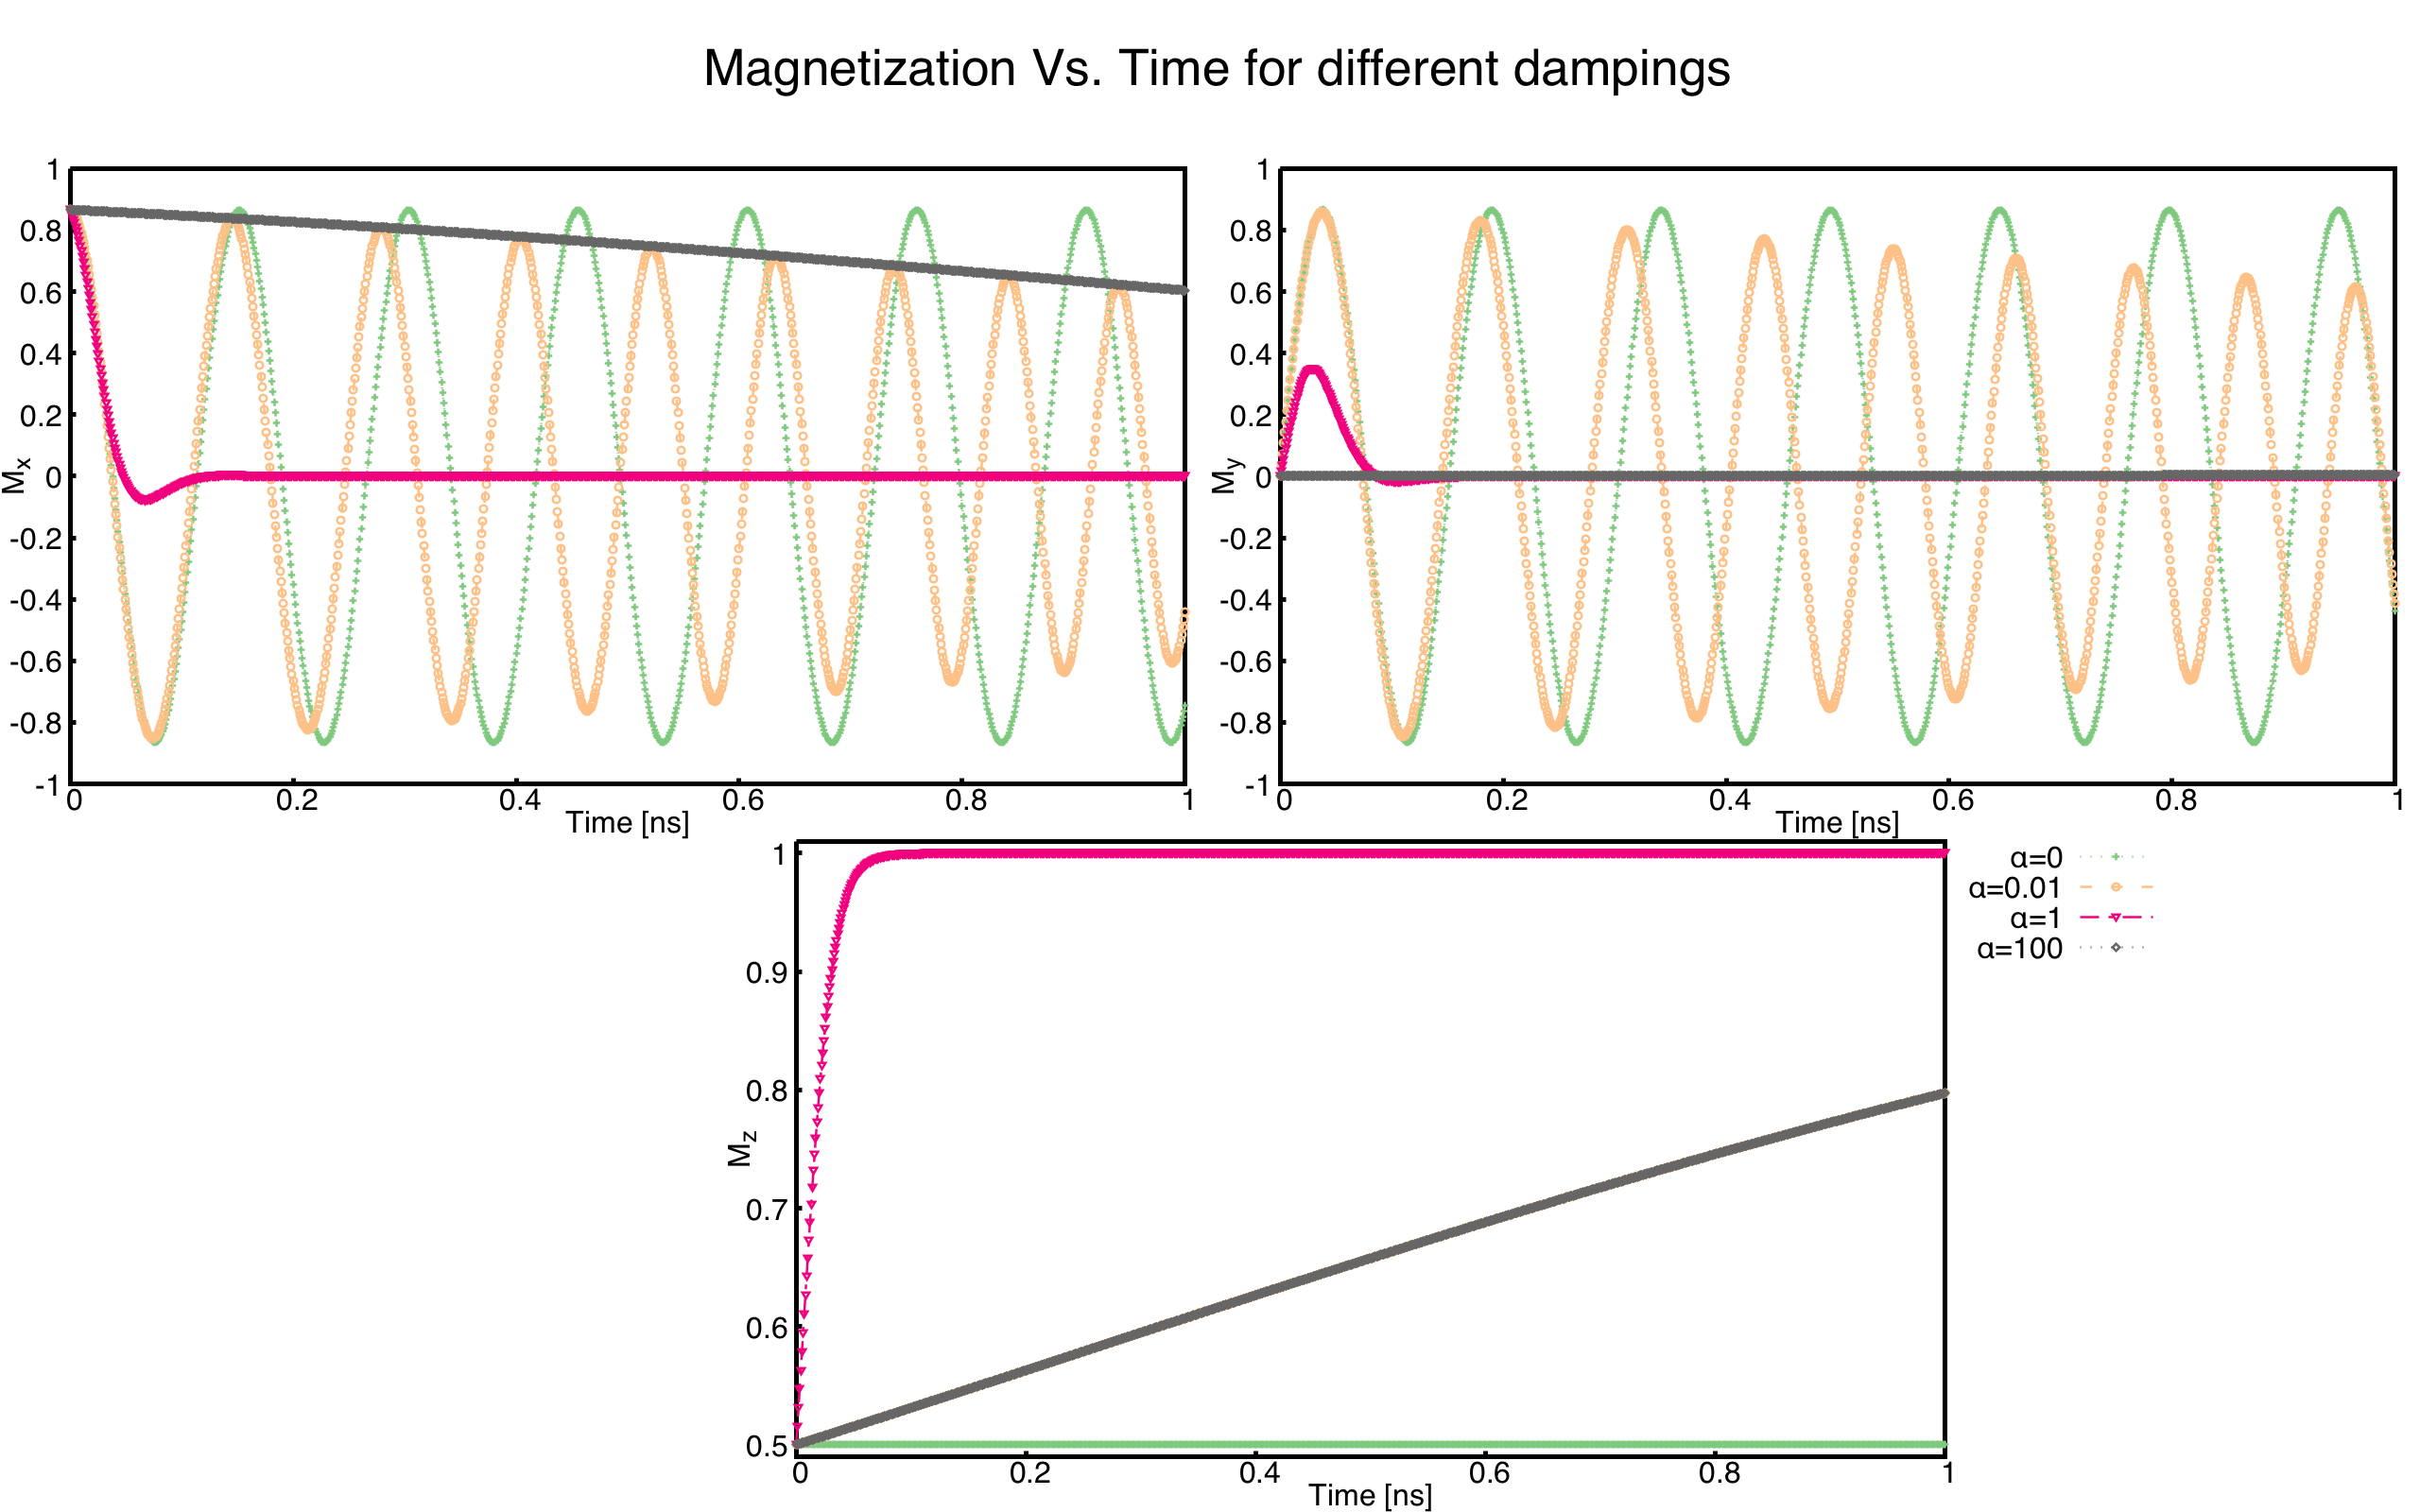
\includegraphics[width=\textwidth]{./GilbertTotal.png}
\caption{Time evolution of the different components of a magnetic moment interacting with the field created by an uniaxial anisotropy when different damping values are considered.\label{fig:Gilbert}}
\end{figure}

As can be seen in this plot one has the time evolution of the different components of the magnetic moments. In general in the limit of low dampign $\alpha<1$ one can see that as the damping increases the system reaches the equiblibrium faster. It is of special interest to also look at the limit $\alpha=0$, where one can see that without damping the spin will prescess around the effective field without ever aligning itself with it, this is evident by looking at the time evolution of $M_z$. However, in the high damping limit $\alpha>1$ as the damping increases the magnetic moment actually slows down, this is of great importance and it is the reason why Gilbert introduced the damping in a different way than Laundau and Lifshitz originally did, as the damping acts as a viscous force, and in the infite damping limit the spin whould not be able to move.

\subsection{Switching under external magnetic field}

Now that the effect of the damping on the dynamics is understood, another aspect of great relevance for magnetization dynamics can be studied, namely the switching of the magnetic moment under the influence of an external field. For this one can run the script \verb;SWEEP_FIELD.sh;

\begin{fBox} 
\begin{Verbatim}
./SWEEP_FIELD.sh
\end{Verbatim}
\end{fBox}

This will create a series of folders named \verb;FIELD{value of the field};, in each of these folders the temperature is set to $T=0\,\textrm{K}$, and the damping is set to $\alpha=0.1$. To observe the switching an external magnetic field is added in the following way

\begin{fBox} 
\begin{Verbatim}
hfield   0.00  0.00  -hfield
\end{Verbatim}
\end{fBox}

\noindent that is, the external field is along the negative z-direction which will extert a torque over the magnetic field.

To study the effect that the external magnetic field has over the dynamics of the system lets use the script \verb;plotB.gnu;

\begin{fBox} 
\begin{Verbatim}
gnuplot plotB.gnu
\end{Verbatim}
\end{fBox}

\noindent this produces a plot named \verb;Switching.png; in it one can see the time evolution of the $M_z$ component for different magnitudes of the external magnetic field. In it one can see that after a certain critical value of the external magnetic field, the magnetic moment switches, going from tending to align itself to the possitive z-direction to the negative z-direction, i.e. using an external magnetic field one can switch the direction of the magnetic moment. 

\begin{figure}[ht]
\center
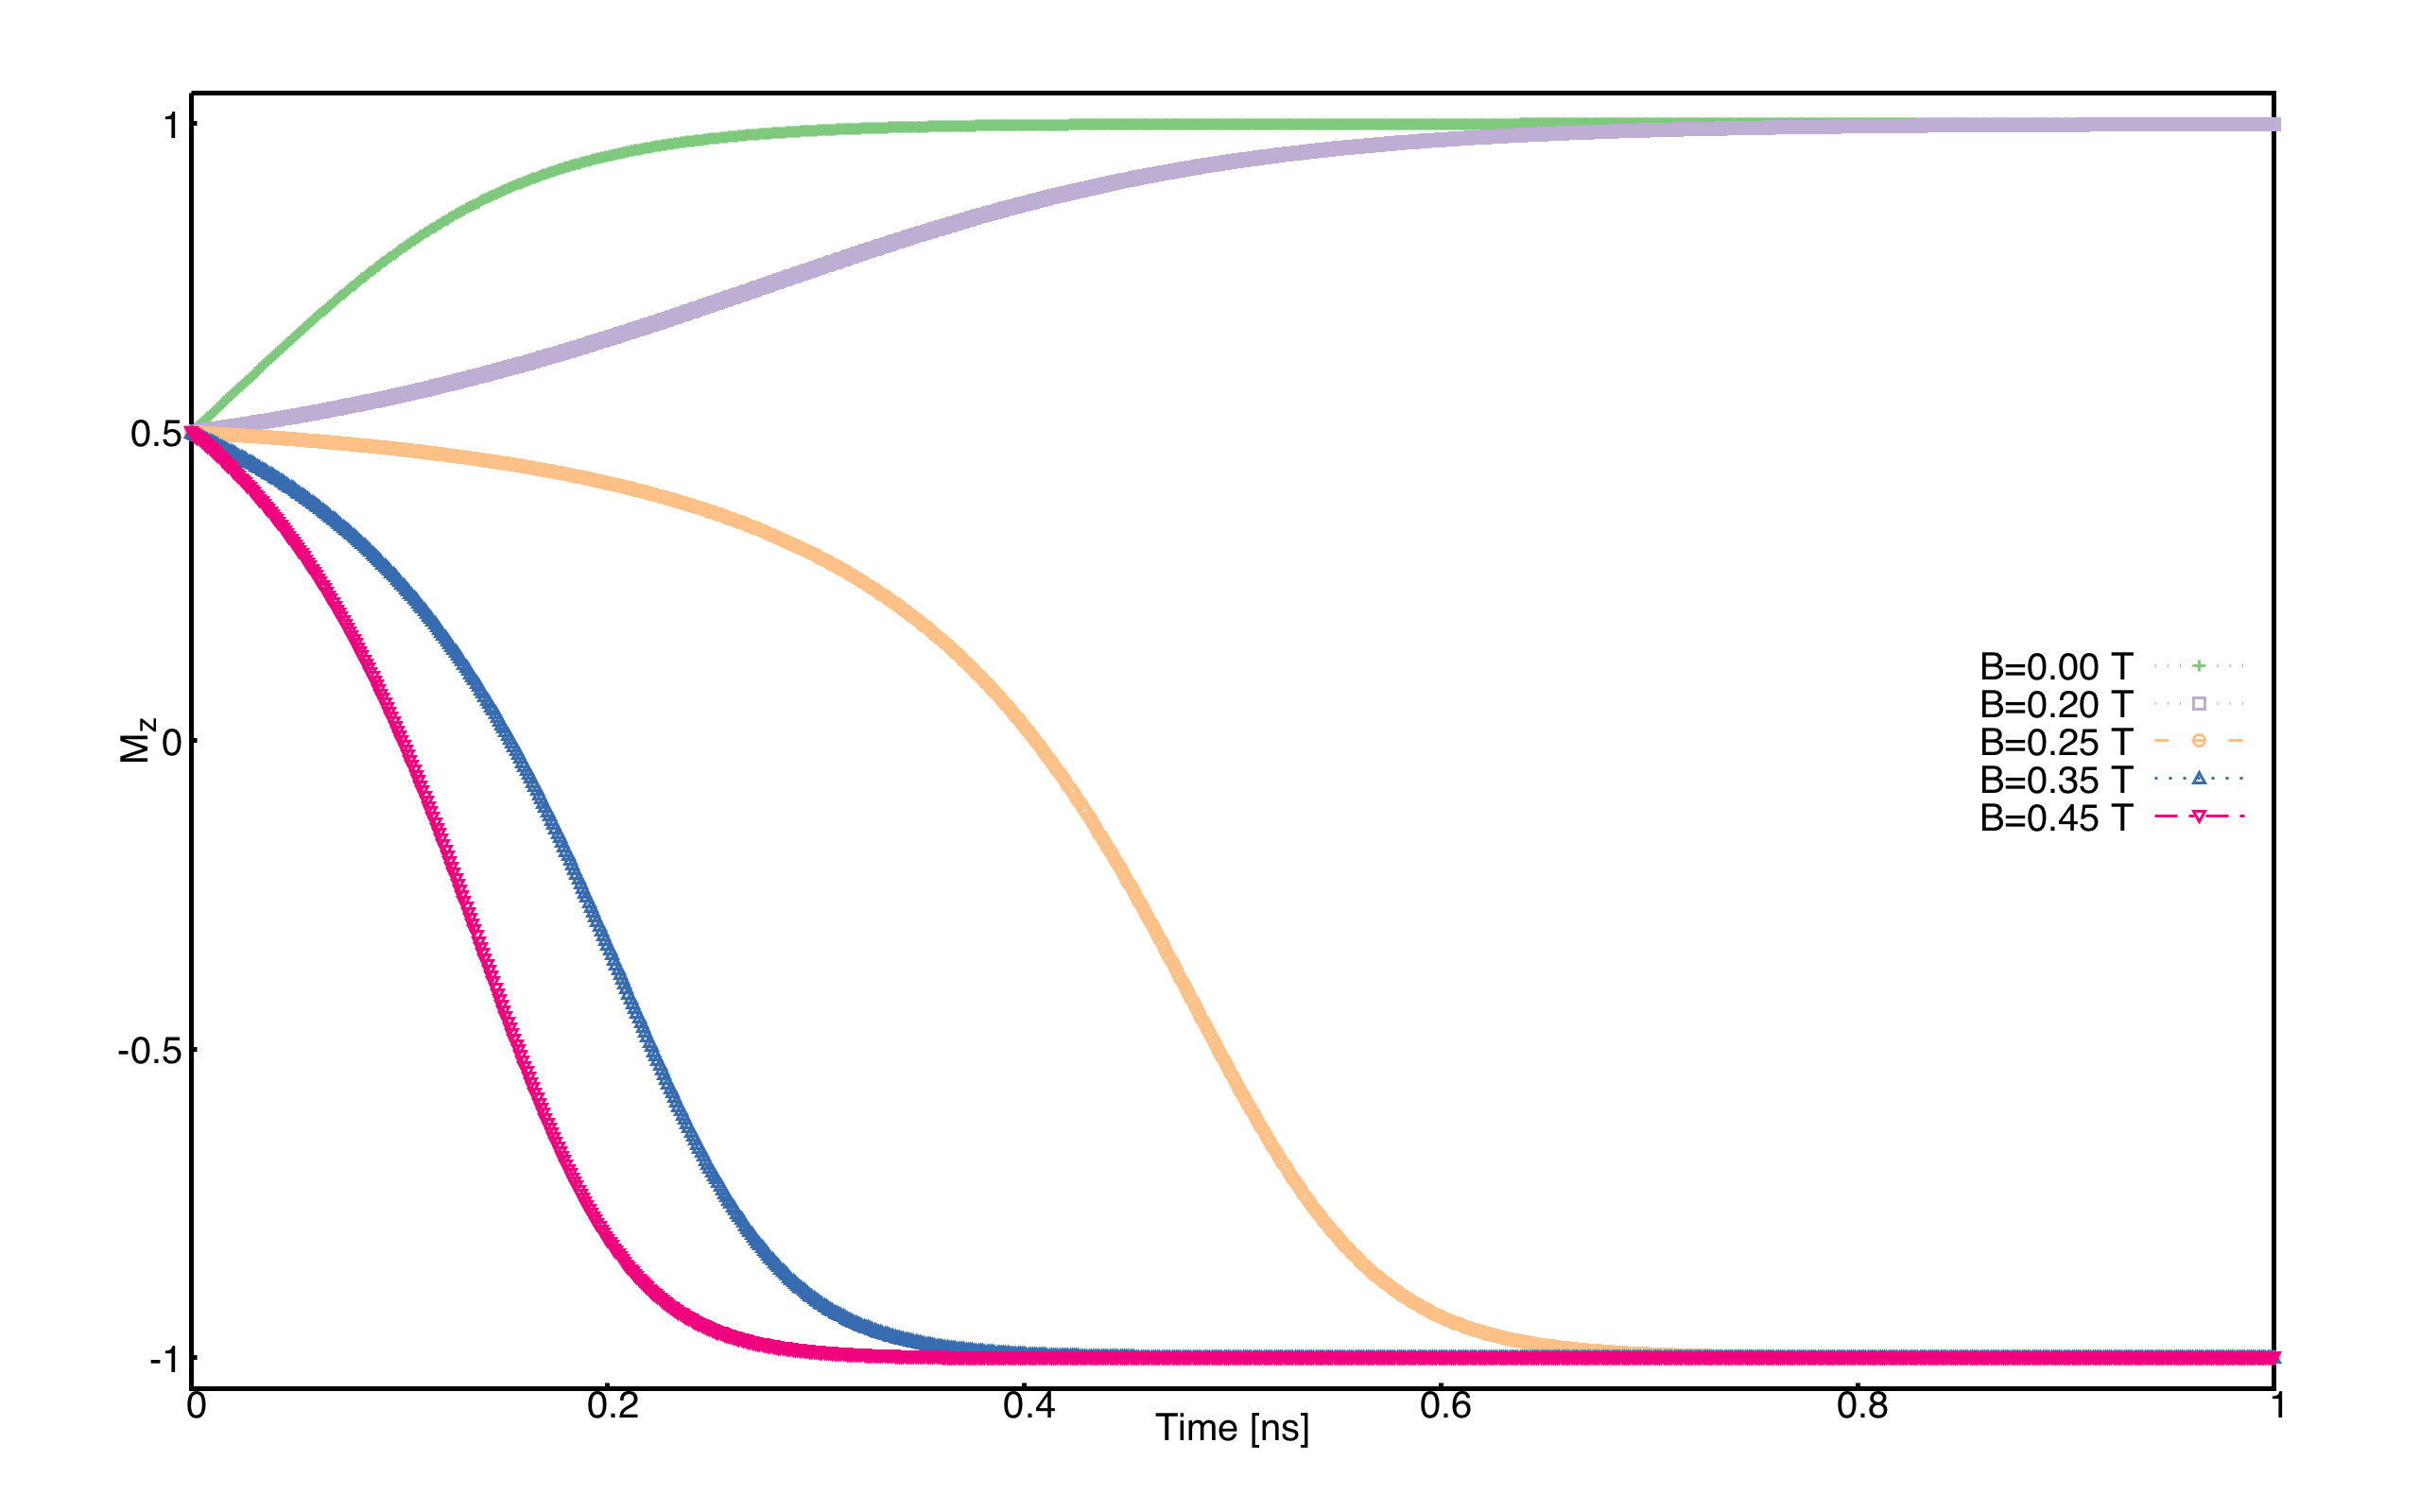
\includegraphics[width=0.75\textwidth]{./Switching.png}
\caption{Time evolution of the $M_z$ component of the magnetic moment under the influence of an external magnetic field of different magnitudes.\label{fig:switching}}
\end{figure}

\subsection{Thermal effects}

Temperature is known to have great importance on the magnetic properties of materials, and henceforth in the dynamics of the magnetic moments. In this section of the tutorial the switching of a magnetic moment thanks to thermal fluctuations. This can be done by running the \verb;SWEEP_TEMP.sh; script. 

\begin{fBox} 
\begin{Verbatim}
./SWEEP_TEMP.sh
\end{Verbatim}
\end{fBox}

The simulations that will be perfomed by this script are very similar to the previous ones, in this case one has a spin aligned along the positive z-direction with a magnetic easy axis along the z-direction. The damping for all these examples is set to $\alpha=0.01$ and the temperature is varied. An analysis of some of the key features of the influence of thermal fluctuations can be observed by using the plotting script \verb;plotTemp.gnu;, this script will generate a couple of plots. Hence one must run the script


\begin{fBox} 
\begin{Verbatim}
gnuplot plotTemp.gnu
\end{Verbatim}
\end{fBox}

First lets study the one called \verb;singleTemp.png;, an example of this can be seen in Fig.~\ref{fig:telegraph}, in which one can see how the spin tends to fluctuate between two orientations ($+z$ and $-z$), this is due to the uniaxial anisotropy present in the system in conjuction with the thermal fluctuations, which allow the spin to overcome the energy barrier given by the anisotropy.

\begin{figure}[h!]
\center
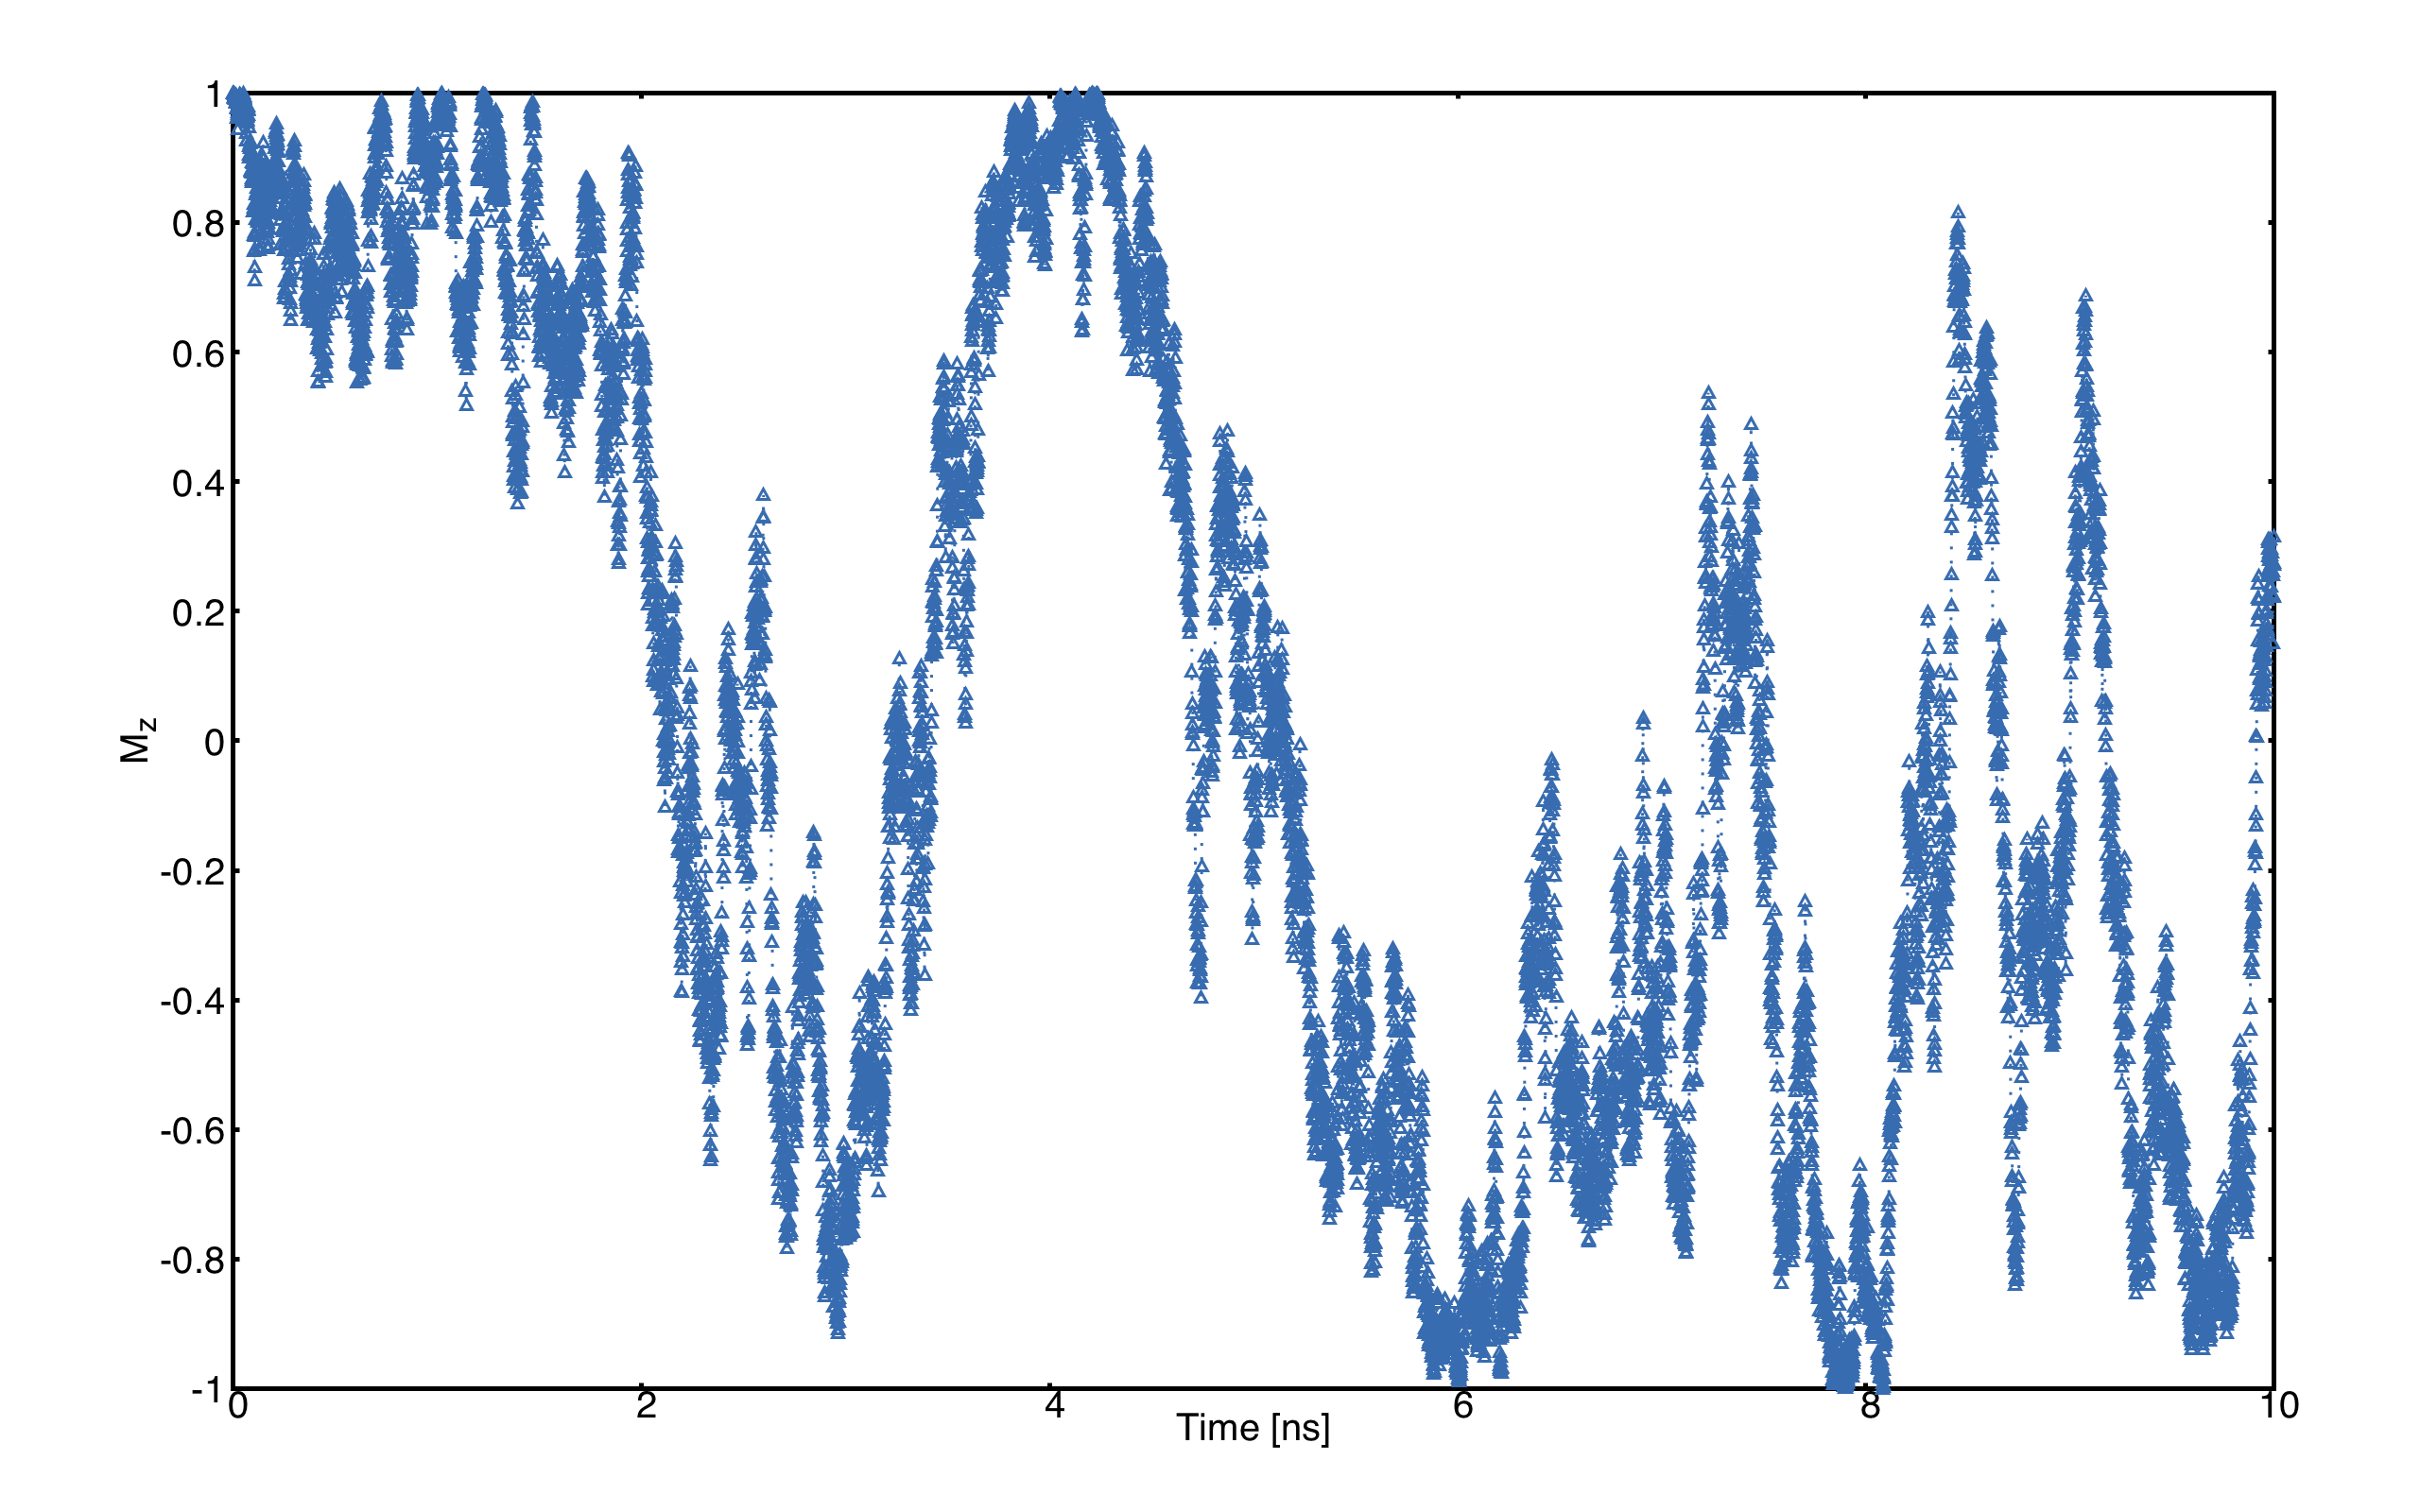
\includegraphics[width=0.75\textwidth]{./singleTemp.png}
\caption{Time evolution of the $M_z$ component of a magnetic moment at $T=4\,\textrm{K}$. \label{fig:telegraph}}
\end{figure}

The next plot named \verb;relaxation.png; is an average over 200 replicas (\verb;Mensembe 200;) of the simulation which are then averaged over. In here one can see instead the average relaxation time of the spin, showing how it can vary with temperature, thus showcansing the importance of 

\begin{figure}[h!]
\center
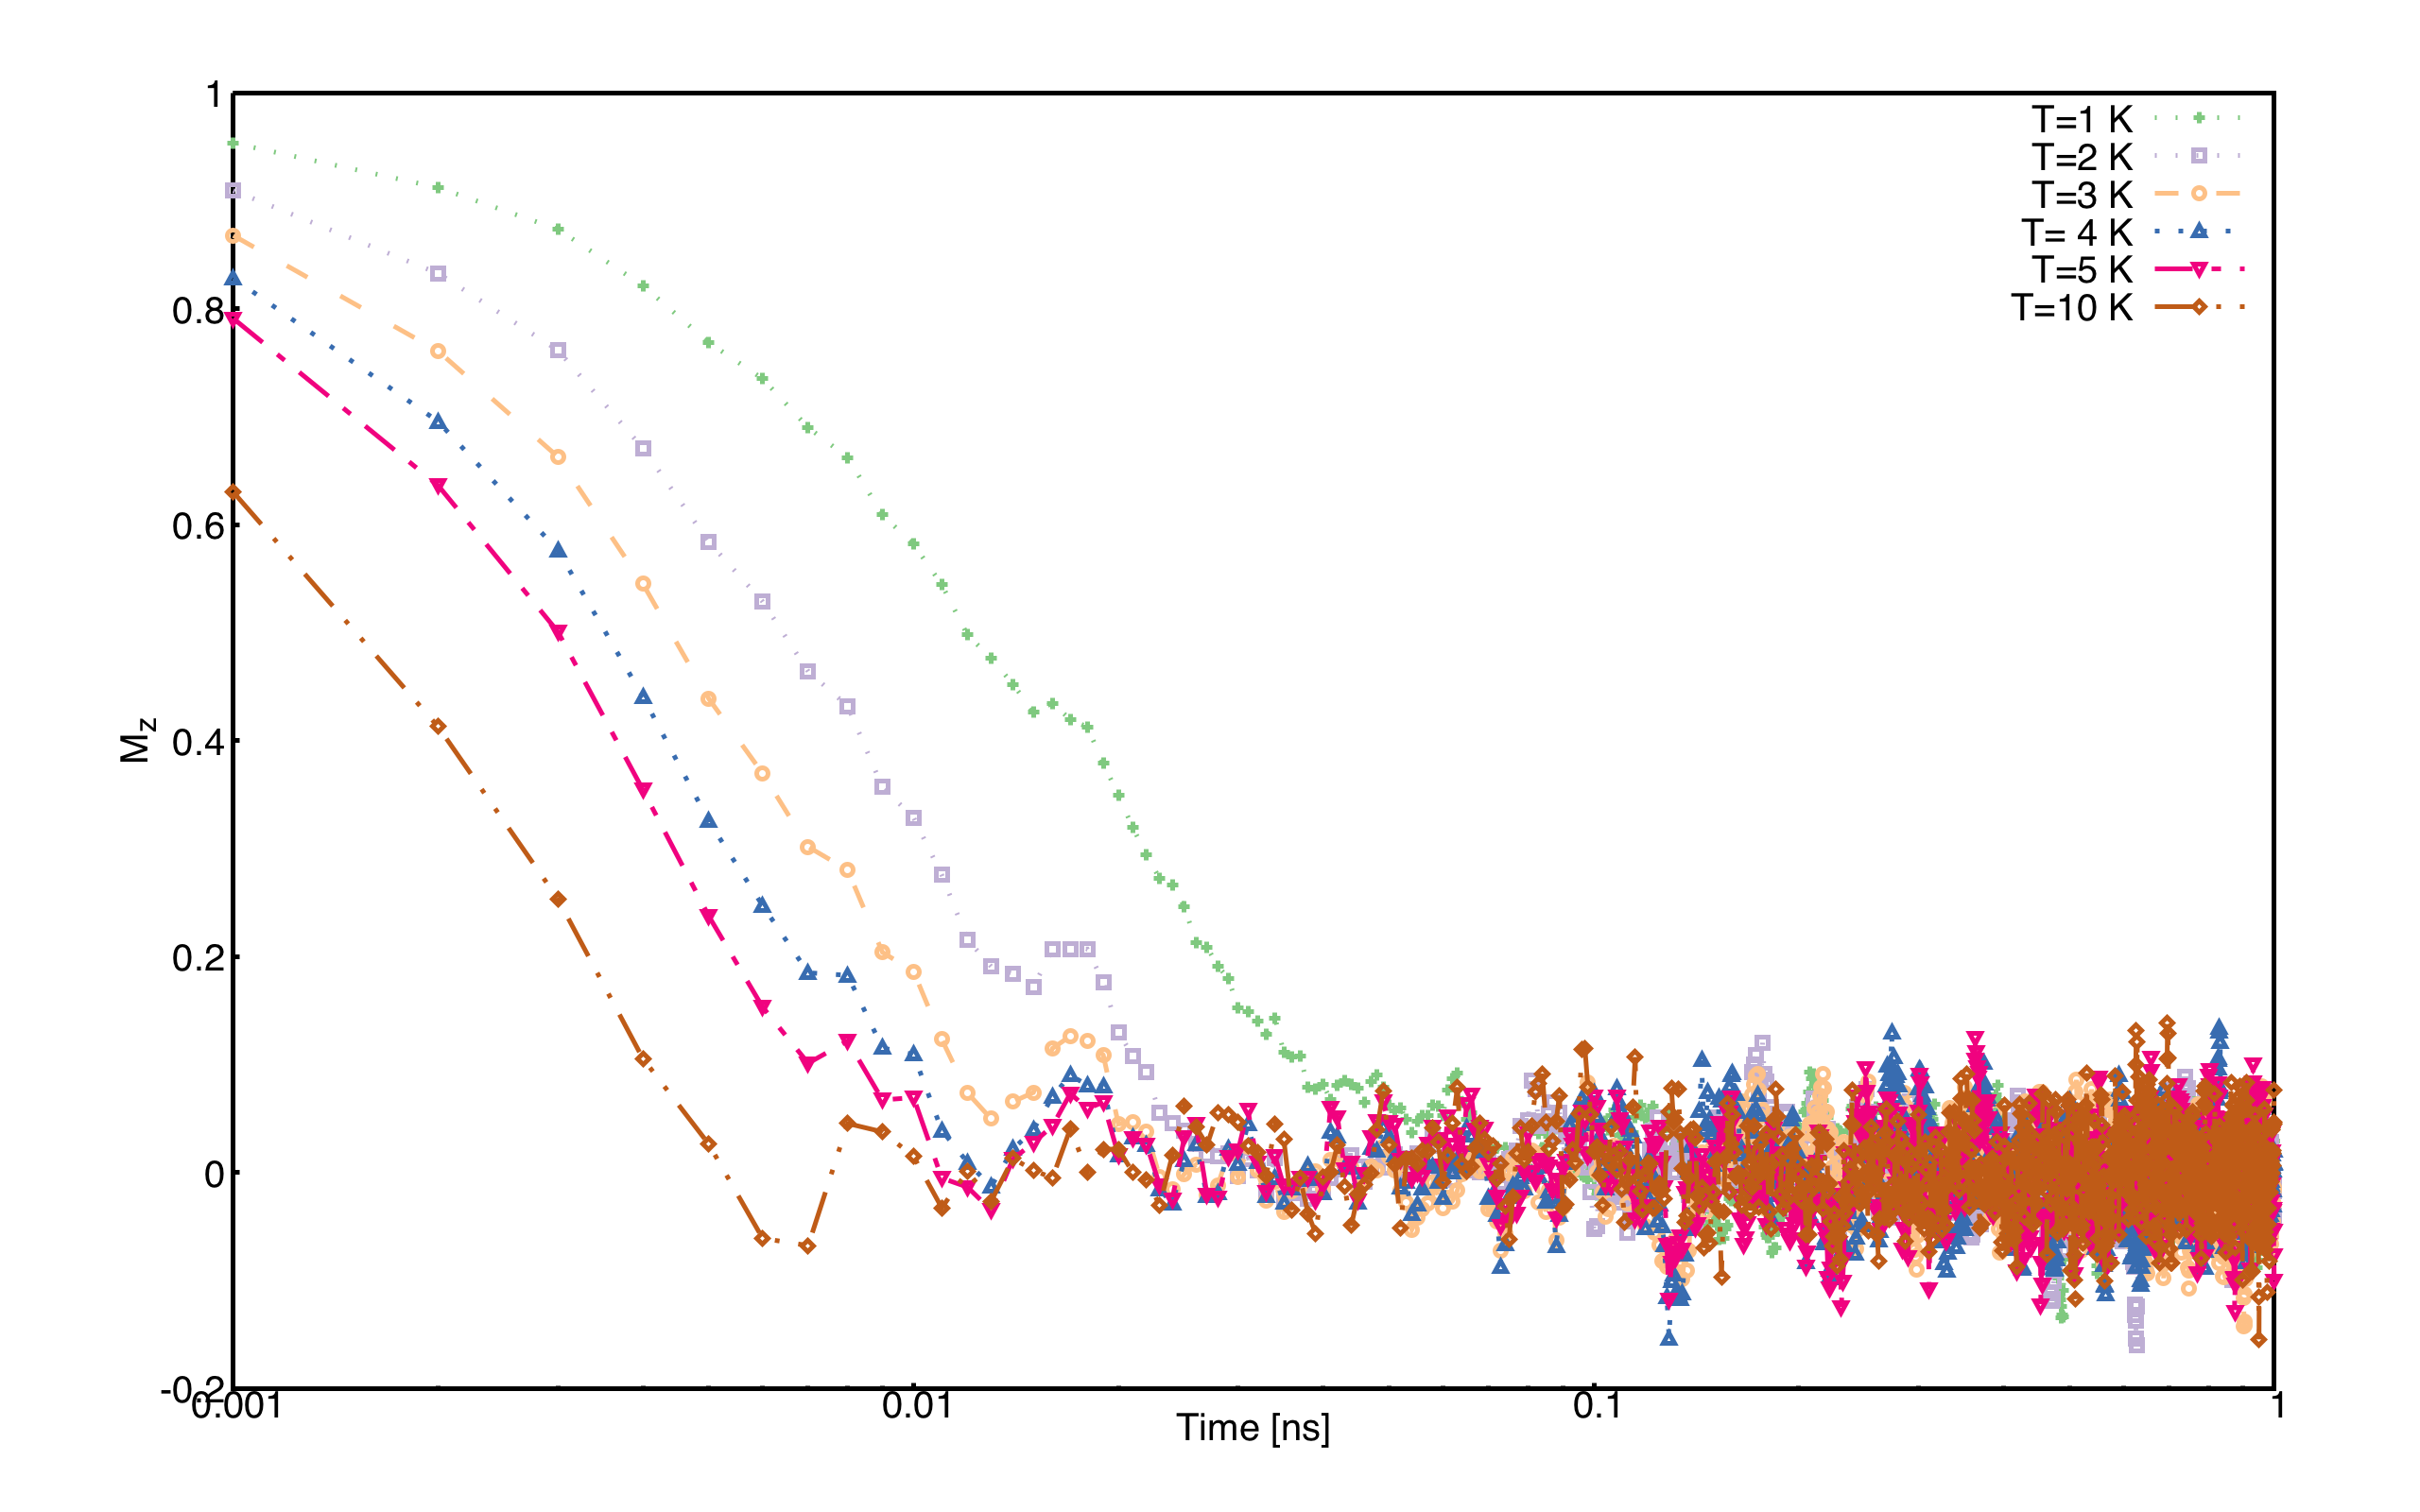
\includegraphics[width=0.75\textwidth]{./relaxation.png}
\caption{Average time evolution of the $M_z$ component of a magnetic moment for several temperatures. \label{fig:relaxation}}
\end{figure}

\section{Determination of T$_c$ of a ferromagnetic material}
When one talks about a ferromagnetic material, one refers to a class of substances that have as a ground state ($T=0\,\textrm{K}$) all its spins aligned in the same direction. As temperature increases disorder enters to the system until at a certain critical (Curie) temperature $T_c$  the system has no net magnetization. The Curie temperature could be seen as the highest possible working temperature for the material and is of great importance for applications.

In this walkthrough we will use Monte Carlo simulations to determine the magnetization as function of temperature and from that the $T_c$. Overall, the procedure is as follows:

\begin{enumerate}
\item Run Monte Carlo simulations using either Metropolis algorithm (\verb;mode M;) or Heat bath algorithm (\verb;mode H;) for a set of different temperatures.
\item Collect the results and analyse the temperature dependent magnetization and/or other thermodynamic properties
\item Determine $T_c$
\end{enumerate}

For this step-by-step walkthrough, we will use the input files for Fe as example that is found in the example directory and displayed in Chapter 2. 

First of all, standing in the root directory, navigate to the input files of Fe:
\begin{fBox} 
\begin{Verbatim}
cd examples_revision_controlled/Fe
\end{Verbatim}
\end{fBox}
The program works in such a way that we need to repeat simulations for different temperatures. For the purpose, it is recommended to use a script that does simplify a lot of things but first we need to prepare the input files for that. We will create a "Base" directory where the raw input files are stored.
\begin{fBox} 
\begin{Verbatim}
mkdir Base ; mv * Base/ 
\end{Verbatim}
\end{fBox}
Next, we need to copy two run-scripts (runme.sh and printM.sh)  that will run a set of simulations at different temperatures from the scripts-directory:
\begin{fBox} 
\begin{Verbatim}
cp ../scripts/runme.sh . ; cp ../scripts/printM.sh .
\end{Verbatim}
\end{fBox}
Before starting the run-scripts, the inpsd.dat file needs to be prepared in such a way that the temperature in both initial and measurement phase are set to "TEMP". Using any editor of choice, change temperature from "300" to "TEMP" of lines 25 and 28. With that, everything is prepared to run the simulations using the run-script:
\begin{fBox} 
\begin{Verbatim}
./runme.sh
\end{Verbatim}
\end{fBox}
Depending on computer system, it may take some time to run through all temperatures. After all calculations are finished, a new directory for each temperature has been created with output files for that particular temperature. To create a summary, we are using the other script (printM.sh) that reads certain information in output files and collect them in a single file (thermal.dat) using the command:
\begin{fBox} 
\begin{Verbatim}
./printM.sh
\end{Verbatim}
\end{fBox}
Let's investigate the generated thermal.dat file.
\begin{fBox} 
\begin{Verbatim}
# Temp.   Mavg     UBinder    Susc.      Cv
    10  2.237941  0.666667  0.000007  1.021710
   100  2.164441  0.666664  0.000071  0.976500
   200  2.078111  0.666654  0.000166  1.024818
   300  1.986299  0.666631  0.000275  1.048131
   400  1.886474  0.666586  0.000422  1.079090
   500  1.777491  0.666515  0.000563  1.172849
   600  1.650539  0.666357  0.000827  1.277333
   700  1.504614  0.666068  0.001138  1.492052
   800  1.308315  0.665102  0.001981  1.770288
   900  1.007354  0.658843  0.005374  2.151073
   950  0.749161  0.635858  0.012374  2.260679
  1000  0.415532  0.542287  0.015266  1.487550
  1050  0.267658  0.473693  0.008910  1.004156
  1100  0.204595  0.442776  0.005369  0.784146
  1150  0.171373  0.429213  0.003673  0.670025
  1200  0.151207  0.444319  0.002641  0.556371
  1250  0.137225  0.455091  0.002093  0.471770
  1300  0.128381  0.431053  0.001813  0.418473
  1500  0.102811  0.464573  0.000898  0.283877
\end{Verbatim}
\end{fBox}
The contents of the file are as follows: first column list the temperature, magnetization (in Bohr) in the second column, the Binder cumulant (see below) in the third column, the susceptibility are found in the fourth columns and the fifth column contains the specific heat (in units of k$_B$). If the magnetization (col 1) is plotted against the temperature (col 1) we immediately see that T$_c$ is around 1000 K. That is also reflected in the peak of the susceptibility (col 4) and the specific heat (col 5) around that temperature. However, in order to obtain a more precise value of T$_c$, the cumulant crossing method that originally was suggested by Binder is very powerful and useful technique. The (4'th order) cumulant U$_L$ , defined as:
\begin{equation}
U_L = 1 -\frac{\langle M^4 \rangle}{3 \langle M^2 \rangle ^2 }
\end{equation}
has unique properties that makes it easy to locate T$_c$ without resorting to advanced finite size scaling analysis or calculation of critical exponents of the transition. As the system approaching infinite size, $U_4 \to 4/9$ for $T> T_c$ and $U_4 \to 2/3$ for $T< T_c$. However, the crucial part is for large enough systems, the curves of $U_4$ for different lattice sizes cross in a fixed point $U^*$ and the location of the fixed point is T$_c$. Practically, that means that all simulations are repeated using some other lattice size of the simulation box. As an example, change the ncell keyword in the inpsd.dat file (line 2) in the Base directory from using a cube of size 12 to 20 (i.e 20 20 20) and repeat the calculations once again using the runme.sh script. Since the simulation box is now larger, it will take longer time to finish (with all other parameters fixed, the simulation time scales linearly with number of atoms in the cell, i.e. $(20/12)^3 \approx 4.6$ longer execution time than previous). Once finished, gather and collect the output using the printM.sh script. Now plot the cumulant as function of temperature and one get a figure similar to as shown in Fig.~\ref{fig:MTFe}. There are some statistical noise at high temperatures which can be reduced by running the simulations with more steps and more ensembles. Nevertheless, there is a distinct crossing around 955 K which is the calculated T$_c$ for the specific system.

\begin{figure}[h!]
\subfloat{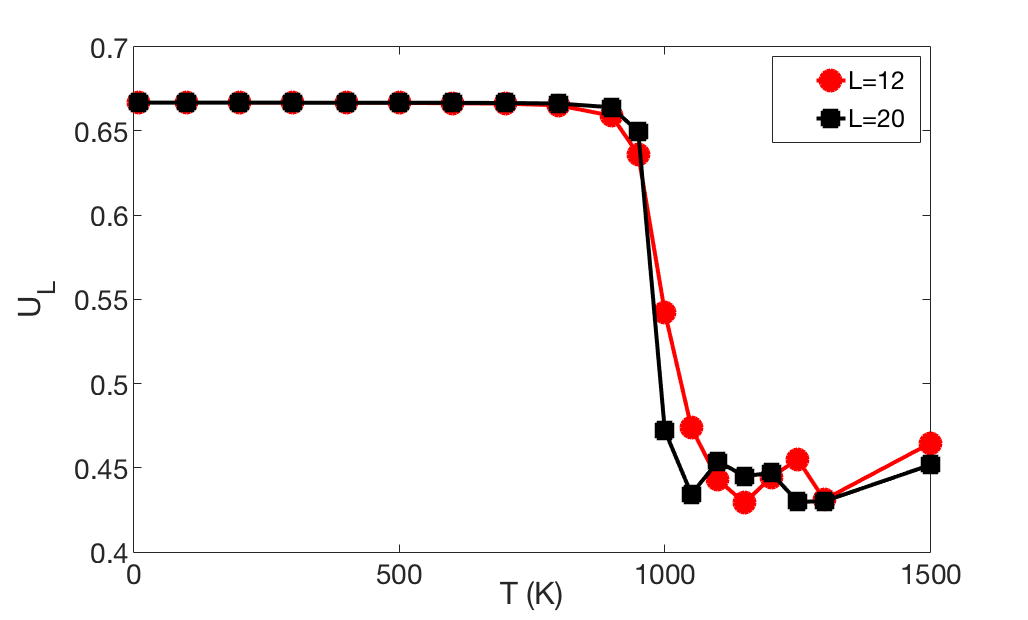
\includegraphics[clip,width=0.49\columnwidth]{./MTFe.png} }\subfloat{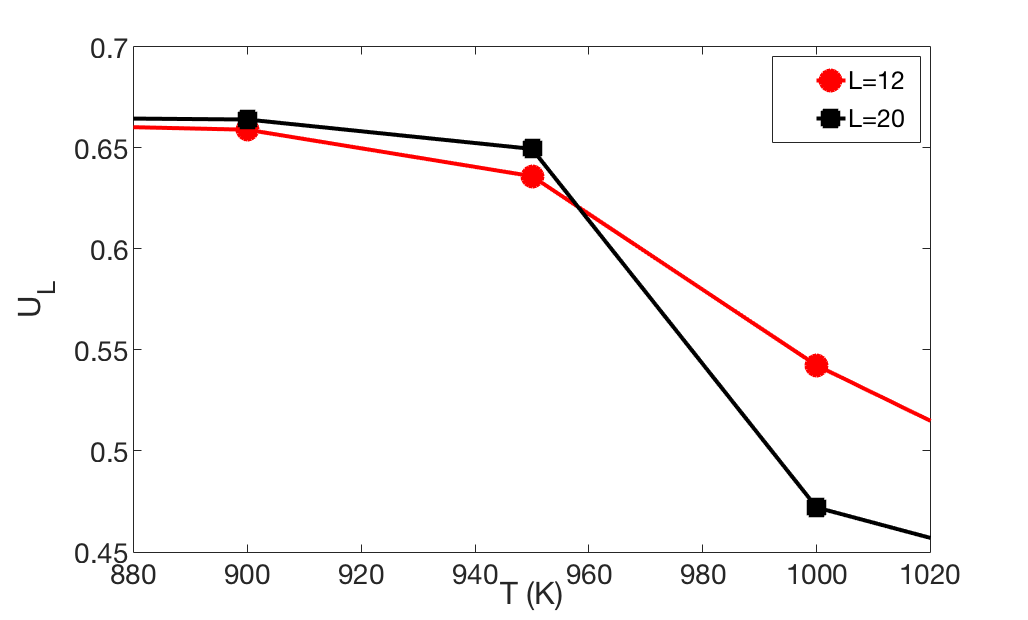
\includegraphics[clip,width=0.49\columnwidth]{MTFe2.png} }
\caption{(left) Cumulant of Fe as function of temperature using cubic simulation box of size L=12 and L=20.  (right) Zoom in of the crossing point and the location of T$_c$.}
\label{fig:MTFe}
\end{figure}

\section{Dynamical correlations and magnon spectra}
A very useful functionality of UppASD is the possibility to simulate the dispersion relations for magnons. This is done by sampling the dynamical structure factor $S(\mathbf{q},\omega)$, as introduced in Sec.\ref{sqw}. The simulated magnon dispersion relations, or magnon spectrum, can straightforwardly be compared with experimental inelastic scattering measurements as a benchmark of the theoretical model. 
%
\subsection{Ferromagnetic magnons}
In this tutorial we will show how to obtain the magnon spectra from ASD simulations of $S(\mathbf{q},\omega)$ as well as from linear spin wave theory, which gives the zero-temperature adiabatic magnon spectra of the same Hamiltonian used for the ASD simulations. The tutorial uses the simple example of a 1d-Heisenberg spin chain found among the examples provided with the UppASD distribution. 
\begin{fBox} 
\begin{Verbatim}
cd examples_revision_controlled/HeisChain
\end{Verbatim}
\end{fBox}
There, the input file \texttt{inpsd.dat} can be inspected and the following lines controls the sampling of the correlation function.
\begin{fBox} 
\begin{Verbatim}
do_sc Q                     
sc_window_fun  2          
do_sc_local_axis N      
sc_local_axis_mix  0.0  

sc_nstep 2000     
sc_step 10        

qpoints F         
qfile   ./qfile
\end{Verbatim}
\end{fBox}
Checking the given parameters with their description in Seq.~\ref{sqw}, we see that here the sampling will be performed with a Hann windowing function, without transforming the system to a local reference frame and with q-points given by the external file \texttt{qfile}. Simulating the system as-is gives a magnon spectrum that looks as the left panel of Fig.\ref{fig:sqw_heischainfm}. In order to visualize the magnon spectrum, scripts are provided both for \texttt{gnuplot} and for \texttt{MATLAB/Octave}. The plot in Fig.\ref{fig:sqw_heischainfm} was obtained by running the script \texttt{Sqw/sqw_map.sh}.
\begin{figure}[h!]
\subfloat{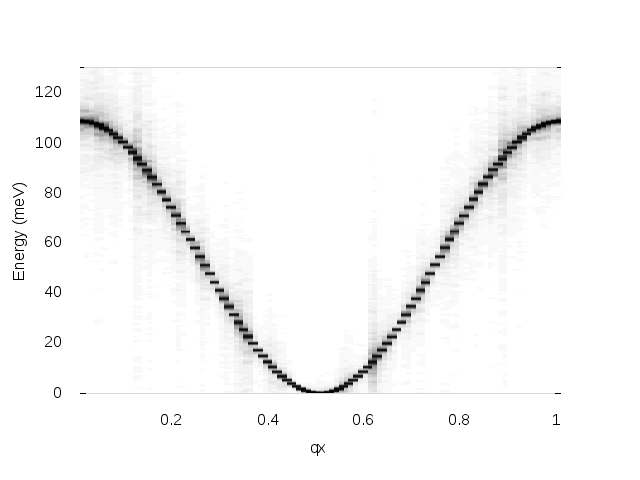
\includegraphics[clip,width=0.49\columnwidth]{sqwheischainfm.png} }\subfloat{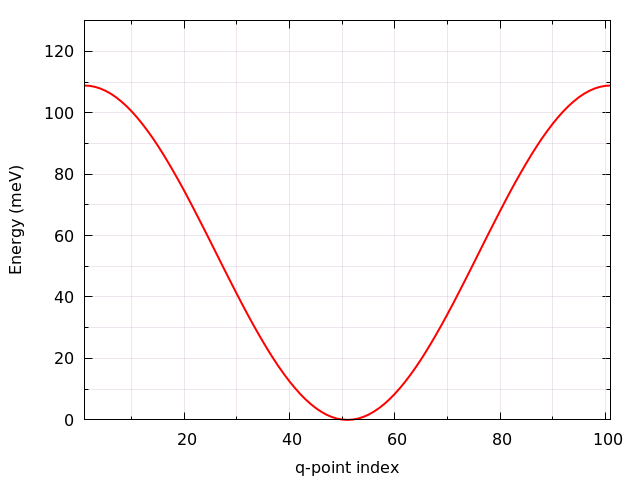
\includegraphics[clip,width=0.49\columnwidth]{amsheischainfm.png} }
\caption{(Left) Simulated magnon spectrum for a ferromagnetic Heisenberg spin chain.
(Right) Adiabatic magnon spectum for the same system.}
\label{fig:sqw_heischainfm}
\end{figure}
In order to get a feeling of which parameters that determine the range and quality of the simulated spectra, it is recommended to change the values of \rkeyword{sc_step}, \rkeyword{sc_nstep}, \rkeyword{sc_window_fun}, and \rkeyword{do_sc_local_axis}. Other general simulation parameters that also affects the $S(\mathbf{q},\omega)$ are also \rkeyword{timestep} and \rkeyword{damping}. Since the simulation window (in the frequency domain) is determined by \rkeyword{timestep}, \rkeyword{sc_step}, and \rkeyword{sc_nstep}, these parameters can be varied to get as efficient sampling as possible. As an example, a weakly coupled system have low-lying excitations and sampling these takes longer time than high-energy magnons. This can then be achieved by increasing \rkeyword{sc_step} but in these cases it is often possible to increase \rkeyword{timestep} as well, as the effective magnetic field, and the resulting torques results in slower precessions of the system and thus a coarser timestep can work. This always has to be tested carefully. The damping strongly affects the magnon spectrum and if a very clean signal is wanted, for careful identification of the magnon energies, then \rkeyword{damping} can be put to a value much lower than what is realistic (i.e. $10^-5$).
\par
An adiabatic magnon spectrum (AMS) can also be obtained by UppASD, in that case put the parameter \rkeyword{do_ams}=y and provide a \rkeyword{qfile} as for the $S(\mathbf{q},\omega)$ simulations. The AMS can conveniently be ran at the same run as $S(\mathbf{q},\omega)$ so that the two different approaches can be compared to each other. By definition, the agreement should be good, and if the two approaches give varying result for a system with low damping and close to zero temperature, then that is a strong indication that either the system is not ferromagnetic or that it might not have been correctly set up. An example of the AMS for the Heisenberg chain is shown in the right panel of Fig.\ref{fig:sqw_heischainfm}. Thanks to the simplicity of this 1d nearest-neighbour model, the AMS can be derived by hand and compared with the simulated results, which is left as an exercise for the reader.
%
\subsection{Magnons in antiferromagnets and spin spirals}
Since the simulated $S(\mathbf{q},\omega)$ only depend on the configurations and trajectories of the simulated magnetic moments, it is not restricted to ferromagnetic systems. Although non-ferromagnetic systems typically needs to be treated a bit more carefully than ferromagnets, it is still possible to obtain magnon spectra for such systems as well. This can be illustrated by running the provided examples \texttt{HeisChainAF} which has anti-feromagnetic exchange interactions, and \texttt{HeisChainDM} which has ferromagnetic interactions but also competing Dzyaloshinskii-Moriya interactions, and compare the output with the previously simulated ferromagnetic Heisenberg chain. Starting with the anti-ferromagnetic system \texttt{HeisChainAF}, running it the same way as the \texttt{HeisChain} example should give the following outputs.
\begin{figure}[h!]
\subfloat{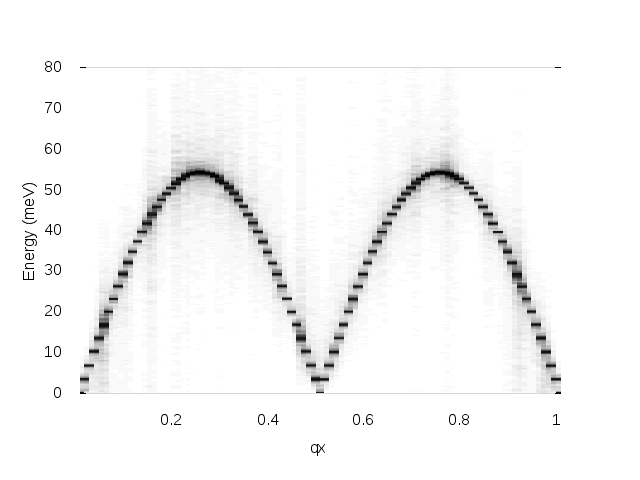
\includegraphics[clip,width=0.49\columnwidth]{sqwheischainafm.png} }\subfloat{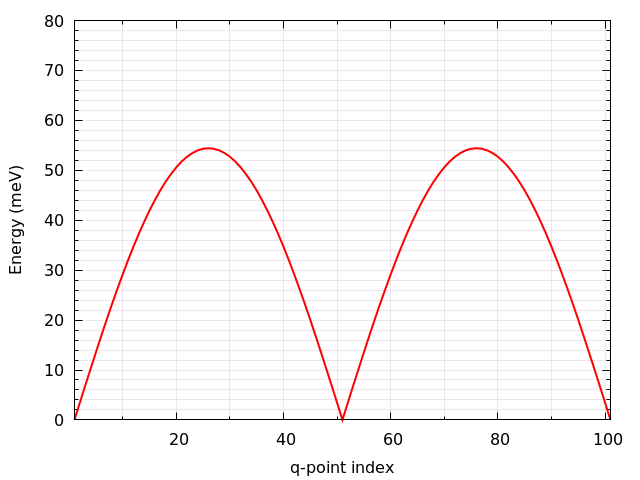
\includegraphics[clip,width=0.49\columnwidth]{amsheischainafm.png} }
\caption{(Left) Simulated magnon spectrum for an anti-ferromagnetic Heisenberg spin chain.
(Right) Adiabatic magnon spectum for the same system.}
\label{fig:sqw_heischainafm}
\end{figure}
Here one can notice the linear dispersion of magnon energies close to the $\Gamma$-point which is always obtained for anti-ferromagnets.
\par
In the \texttt{HeisChainDM} example, the competition between Heisenberg and Dzyaloshinskii-Moriya exchange results in a helical spin spiral with a pitch-vector along $\hat{z}$ and the moments rotate in the $\hat{x}\hat{y}$-plane. The corresponding magnon spectrum is shown in Fig.~\ref{fig:sqw_heischaindm} where it can be noticed that the minimum energy is not found for the $\Gamma$-point but for the q-point $q_0$ corresponding to the wave-vector of the resulting spin spiral. It can also be seen that the agreement between the AMS and $S(\mathbf{q},\omega)$ is good but not perfect here. This highlights the important fact that the AMS currently does not have a general support for treating DMI interactions and while it can be expected to perform well for co-planar spin spirals, as found in this case, it should be handled with care. It can also be noted that the AMS only picks up one of the two non-degenerate magnon branches while both $q^+_0$ and $q^-_0$ are sampled by the $S(\mathbf{q},\omega)$.

For spin spiral systems, the magnon dispersions do not behave as they in collinear systems. Instead there is a much stronger variation of the dispersion relations depending on which axis the excitations are sampled along. This can be observed by changing the \rkeyword{do_sc_local_axis} parameter and compare the simulated spectra. Also, running the \texttt{sqw_map.sh} post-processing script creates a combined figure of the magnon spectra along all cartesian/local axes in the file \texttt{sqw_parts.png} which is plotted for this system in the right panel of Fig.~\ref{fig:sqw_heischaindm}
\begin{figure}[h!]
\subfloat{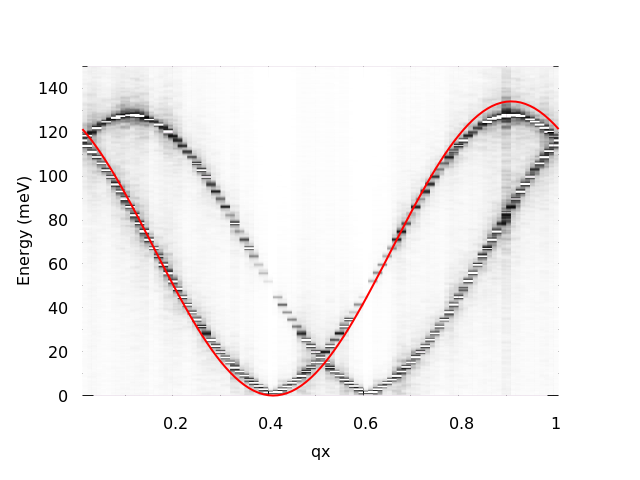
\includegraphics[clip,width=0.49\columnwidth]{sqwamsheischaindm.png} }\subfloat{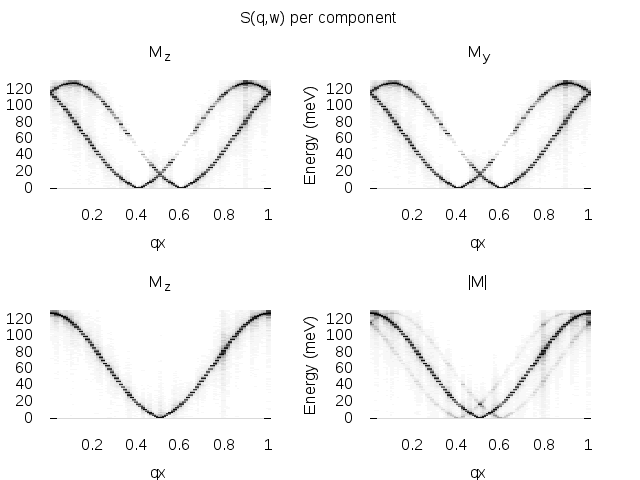
\includegraphics[clip,width=0.49\columnwidth]{sqwcompheischaindm.png} }
\caption{(Left) Simulated magnon spectrum for a Heisenberg spin chain with DM interactions along with the corresponding AMS.
(Right) Projections of $S(\mathbf{q},\omega)$ to the cartesian components $S^\alpha$ and the total magnitude $|S|$ for the same system.}
\label{fig:sqw_heischaindm}
\end{figure}

\chapter{Examples}\index{Examples}
The best way to learn the code is to work through the examples in the directory \texttt{examples}. The current set of examples illustrates the range of the functionality of UppASD, and gives a feel for the data analysis that is necessary in order to interpret the results of the simulations.

\subsection{bcc Fe}
The \texttt{bccFe} directory contains the necessary input in order to simulate bcc Fe. There are a couple of Matlab scripts enclosed that plot quantities such as the average magnetization as a function of time. By varying input parameters such as the temperature, one may get a feel for how these affect these observable quantities.

The \texttt{bccFe-Tsweep} directory contains very similar input to the \texttt{bccFe} directory. However, a small wrapper is included in order to run SD simulations as a function of temperature. This is often useful for checking the transition temperature of a given system. 

%%%%%%
\subsection{Heisenberg Spin Chain}
The \texttt{HeisChain} directory contains possibly the simplest system that can be set up with UppASD: a Heisenberg ferromagnetic chain. This example is set up to allow the spin wave spectrum of the system to be probed. Since the dispersion of this system can be derived analytically (as discussed any many textbooks concerning solid state physics), it is a handy example to get acquainted with spin correlations and dynamics in UppASD. 

By copying over the \texttt{sqw.simid.out} and \texttt{inpsd.dat} files into the \texttt{Sqw} directory, and running the \texttt{sqw_map.sh} script, $S(q,\omega)$ as a function of $q$ is plotted, giving rise to the spin wave displersion. 
The dynamics of spin waves have been studied in this way in the paper by Bergman \textit{et al.}~\cite{Bergman2010}

%%%%%%
\subsection{Two-dimensional Systems}
The \texttt{2d-systems} directory contains a couple of two-dimensional systems: the surface simulating the Co/Cu(001) monolayer system (\texttt{fcc001}), and the square lattice Heisenberg system (\texttt{sc}, which stands for simple cubic). In the latter example, the flag \rkeyword{aunits} is switched on. By running the simulation as a function of temperature, the magnetization can be benchmarked against data obtained from the ALPS software package\footnote{\url{http://alps.comp-phys.org}}, which is contained in the \texttt{scL64ALPS.dat} file.

For both the \texttt{fcc001} and \texttt{sc} examples, a directory \texttt{Snapshots} is included, that allows snapshots of the lattices to be taken. The scripts are written in VTK, and require \rfilename{coord.simid.out} and \rfilename{moments.simid.out} files to work.

%%%%%%
\subsection{fcc Co}
Another very common structure in solid state physics is the fcc structure. This example allows the measurement of the dyamical structure factor, $S(q,\omega)$, for fcc Co, as in the Heisenberg spin chain example.

%%%%%%
\subsection{GaMnAs}
The \texttt{GaMnAs} directory contains input data that sets up a GaMnAs dilute magnetic semiconductor.

%%%%%%
\subsection{Random Alloy}
The \texttt{Ralloy} directory contains input data necessary to set up a dilute random alloy.

%%%%%%
\subsection{SKKR Input (test)}
The \texttt{xctensortest} directory contains the same data as in the \texttt{bccFe} directory, but set up in the tensorial format that arises from the Vienna-Budapest SKKR code.~\cite{Udvardi2003}


%----------------------------------------------------------------------------------------
%	BIBLIOGRAPHY
%----------------------------------------------------------------------------------------

%\chapter*{Bibliography}
%\addcontentsline{toc}{chapter}{\textcolor{ocre}{Bibliography}}
%\section*{Books}
%\addcontentsline{toc}{section}{Books}
%\printbibliography[heading=bibempty,type=book]
%\section*{Articles}
%\addcontentsline{toc}{section}{Articles}
%\printbibliography[heading=bibempty,type=article]
\begin{thebibliography}{1}

\bibitem{Skubic2008}
B.~Skubic, J.~Hellsvik, L.~Nordstr{\"o}m, and O.~Eriksson\\
%\newblock A method for atomistic spin dynamics simulations: implementations and examples.
\newblock {J. Phys.: Condens. Matter}, \textbf{20},315203, 2008.

\bibitem{Antropov1996}
V.~P. Antropov, M.~I. Katsnelson, B.~N. Harmon, M.~van Schilfgaarde, and
  D.~Kusnezov \\
%\newblock Spin dynamics in magnets: Equation of motion and finite temperature effects.
\newblock {Phys. Rev. B}, \textbf{54},1019, 1996.

\bibitem{Garcia-Palacios1998}
J.~L. Garc\'\i{}a-Palacios and F.~J. L\'azaro\\
%\newblock Anisotropy effects on the nonlinear magnetic susceptibilities of superparamagnetic particles.
\newblock {Phys. Rev. B}, \textbf{ 55},1006, 1997.

\bibitem{Watson1969}
R.~E. Watson, M.~Blume, and G.~H. Vineyard\\
%\newblock Spin motions in a classical ferromagnet.
\newblock { Phys. Rev.}, \textbf{ 181},811, 1969.

\bibitem{Eriksson2017}
O.~Eriksson, A.~Bergman, L.~Bergqvist, and J.~Hellsvik\\
\newblock {\it Atomistic {S}pin {D}ynamics - {F}oundations and {A}pplications}.\\
\newblock Oxford University Press, Oxford, 1st edition, 2017

\bibitem{Lichtenstein1987}
A.I.~Liechtenstein, M.I.~Katsnelson, V.P.~Antropov,  and V.A.~Gubanov\\
%\newblock Local spin density functional approach to the theory of exchange interactions in ferromagnetic metals and alloys.
\newblock {J. Magn. Magn. Mater.}, \textbf{ 67},65, 1987.

\bibitem{Binder2009}
K.~Binder and D.~P. Landau\\
\newblock {\it A {G}uide to {M}onte {C}arlo {S}imulation in {S}tatistical {P}hysics}.\\
\newblock Cambridge University Press, Cambridge, 3rd edition, 2009.

\bibitem{Udvardi2003}
L.~Udvardi, L.~Szunyogh, K.~Palot\'as, and P.~Weinberger \\
%\newblock First-principles relativistic study of spin waves in thin magnetic films.
\newblock { Phys. Rev. B}, \textbf{ 68},104436, 2003.

\bibitem{Mentink2010}
J.~H. Mentink, M.~V. Tretyakov, A.~Fasolino, M.~I. Katsnelson, and {\relax
  Th}.~Rasing \\
%\newblock Stable and fast semi-implicit integration of the stochastic {L}andau-{L}ifshitz equation.
\newblock { J. Phys.: Condens. Matter}, \textbf{ 22},176001, 2010.

\bibitem{Depondt2009}
Ph.~Depondt and F.G.~Mertens \\
%\newblock Spin dynamics simulations of two-dimensional clusters with {H}eisenberg and dipole-dipole interactions.
\newblock { J. Phys.: Condens. Matter}, \textbf{ 21},336005, 2009.

\bibitem{Bergman2010}
A.~Bergman, A.~Taroni, L.~Bergqvist, J.~Hellsvik, B.~Hj{\"o}rvarsson, and
  O.~Eriksson \\
%\newblock Magnon softening in a ferromagnetic monolayer: A first-principles spin dynamics study.
\newblock { Phys. Rev. B}, \textbf{ 81},144416, 2010.

\end{thebibliography}

%----------------------------------------------------------------------------------------
%	INDEX
%----------------------------------------------------------------------------------------

\cleardoublepage
\phantomsection
\setlength{\columnsep}{0.75cm}
\addcontentsline{toc}{chapter}{\textcolor{ocre}{Index}}
\printindex

%----------------------------------------------------------------------------------------

\end{document}
